\title{Method}

In this chapter we will shed light on the path we took, the decisions we made, and the progression of our project, with a primary focus on the architectures that underpinned our work.\\

Before proceeding to suggest potential architectures to our client, our initial task involved the selection of appropriate hardware and software, which we then integrated into a range of architectural designs and presented to the client, allowing them to further specify which configurations were the most interesting to their intended usage. This section aims to give an overview of the breadth of options we considered before narrowing down our focus.\\

%Before we could present a set of potential architectures to our client, our first step was to select desired hardware and software. We incorporated the chosen components into different architectural designs which we then presented to our client, allowing them to further specify which configurations were the most interesting to their intended usage. These architectures, which form the initial part of this chapter, will be given a cursory overview. This part aims to give a glimpse of the breadth of options we considered before narrowing down our focus. \\

After thorough discussions and iterations with our client, we arrived at a consensus on the architectures that held the most potential for our client's interests. This agreement marked a significant turning point in our project, as it enabled us to channel our efforts in a focused direction. \\

After deciding which architectures we would proceed with, we will outline and detail the decisions that went into each architectural design. This will give a clear picture of how and why we selected the hardware and software that comprises our system.\\
\newpage

\section{Hardware Selection Process}

In the initial phase of the project, we presented multiple architectural designs to our client from which they chose three different versions, each with slight modifications. KDA expressed interest in an in-depth exploration of sensor readings conducted at the edge, prompting our decision to design a more decentralized architecture. This setup separates functionality between the edge configuration while maintaining a central configuration that remains consistent across all versions.\\

Earlier versions of the Local Hawk drone could fly independently using GPS, an internal measurement unit, and a barometer. These features were enabled by a specific accessory for the Raspberry Pi 4, called a NAVIO2 hat, which provided all the necessary sensors. The drone's flight was controlled by Ardupilot, a software suite running directly on the Raspberry Pi 4. However, our client wanted to avoid overloading the Raspberry Pi 4's processor with the heavy computational tasks associated with object detection. As a result, we were asked to focus on solutions where image processing is carried out on separate, dedicated hardware. Early in the project, we identified and chose various hardware parts that would be appropriate for our drone designs.\\

%----SJEKKE MED MARTIN ---- Prior versions of the Local Hawk Unmanned Aerial Vehicle (UAV) were equipped to navigate autonomously using Global Positioning System (GPS), an Inertial Measurement Unit (IMU), and a barometer. This capability was facilitated by a NAVIO2 hat for the Raspberry Pi 4, which supplied all necessary sensors. The UAV flight control software suite, Ardupilot, operated directly on the Pi 4. However, KDA sought to avoid burdening the Pi 4's CPU with heavy computations required for object detection. Thus, we were directed to concentrate on distributed solutions where image processing is executed on dedicated hardware. Early in the project, we identified and selected various hardware components suitable for our UAV architectures.

\subsection{nVidia Jetson Nano}
The Jetson Nano is a single-board computer with a built-in NVIDIA GPU with 128 CUDA cores.
CUDA (Compute Unified Device Architecture) is a parallel computing platform and application programming interface (API) model that utilizes NVIDIA's graphics processing units (GPUs) for general purpose computing. By allowing developers to leverage the power of GPU beyond graphics, CUDA has vastly increased the efficiency and speed of computationally intensive applications. It provides a suite of software tools and libraries that allow developers to create software that can perform complex computational tasks on GPUs, thus significantly improving performance for applications involving mathematical and scientific computations, image processing, and more.\\

We chose the Jetson because the GPU can be leveraged for high-performance deep learning-based object detection. Performing image processing on a GPU has the added benefit of freeing up the CPU for other tasks.\cite{gpudeeplearningperf}\\

\begin{figure}[h]
    \centering
    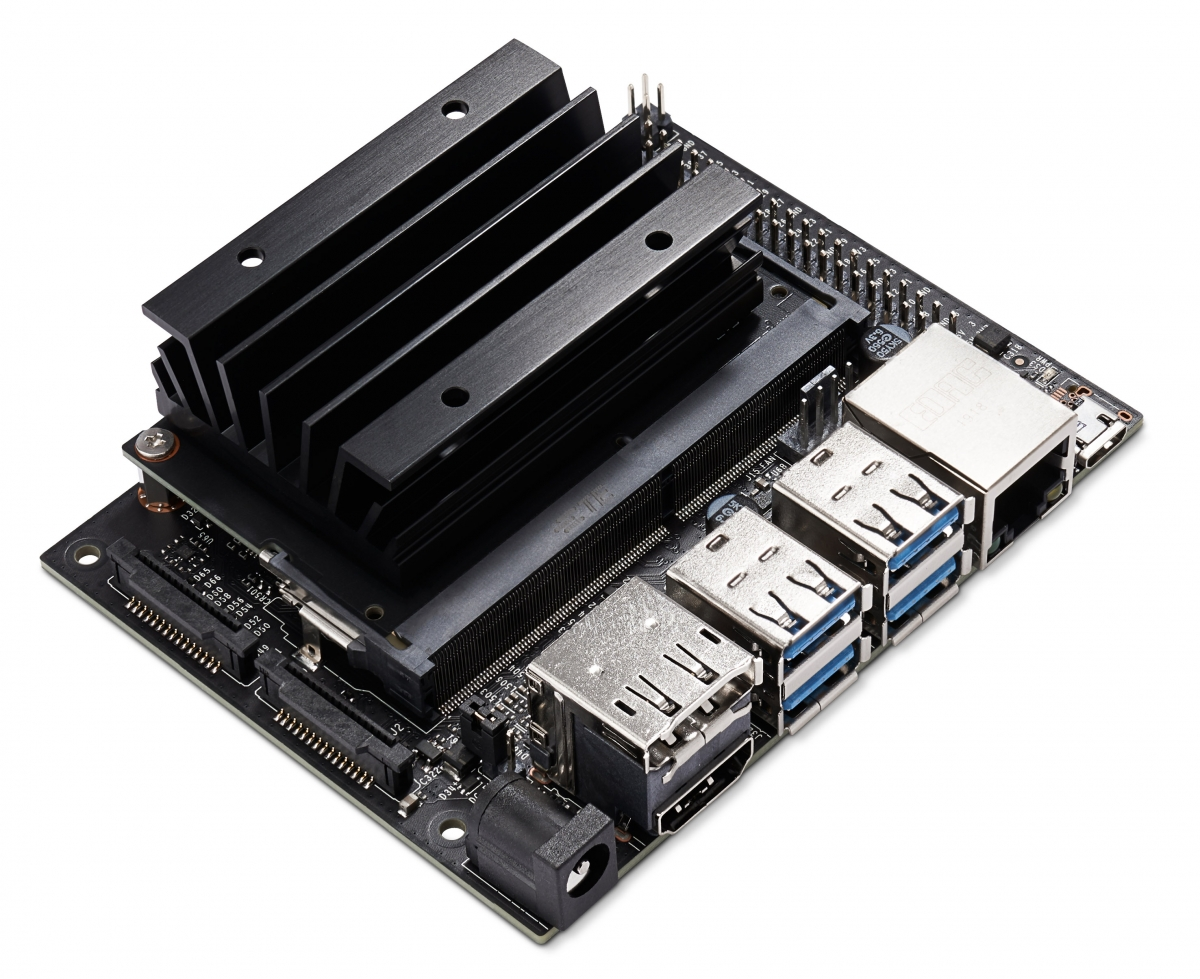
\includegraphics[scale=0.2]{fig/JetsonNano-DevKit_Front-Top_Right_trimmed.jpg}
    \caption{Jetson nano \cite{Jetson}}
\end{figure}

\subsection{Coral Edge TPU}
Google's Coral Edge Tensor Processing Unit (TPU) is a type of custom-built circuit known as an "application-specific integrated circuit" or ASIC. This TPU is specifically designed for deep learning inference, which involves making predictions from new data using a trained machine learning model. Similar to the GPU embedded in the Jetson Nano, this hardware is believed to execute object detection based on deep learning more rapidly than a CPU in a typical single-board computer. The Coral Edge TPU is a USB device, meaning it needs a computer to function.\\

Our interest in the Coral Edge was driven by its light weight and compact size. Coupled with a Raspberry Pi single-board computer, it would create a system that is cost-effective and light, ideal for our project requirements. We were keen to explore the performance potential of this hardware combination.\\

\begin{figure}[h]
    \centering
    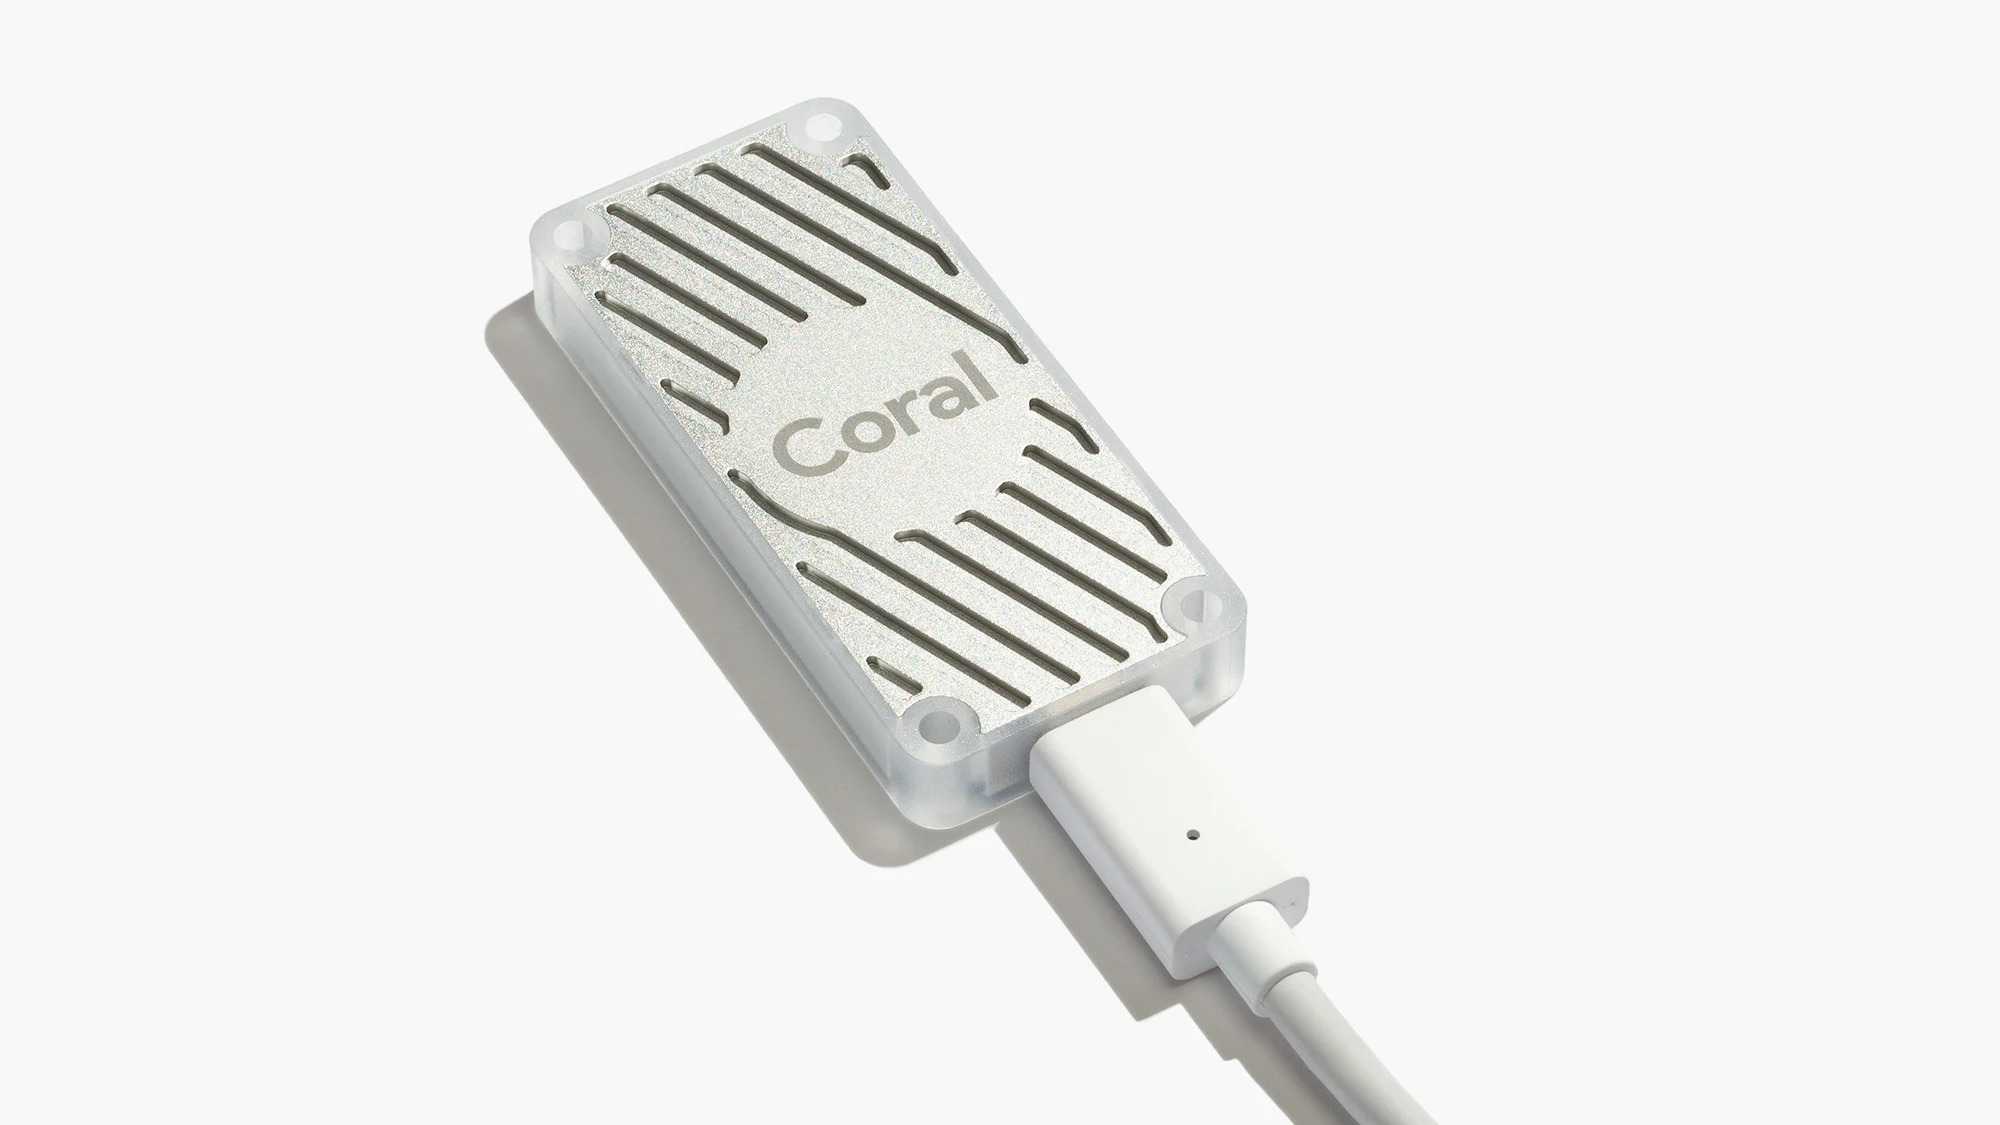
\includegraphics[scale=0.1]{fig/Coral TPU.jpg}
    \caption{Coral USB accelerator \cite{CoralTPU_bilde}}
\end{figure}


\subsection{Raspberry Pi 4B \& Zero 2}

The Raspberry Pi 4B and Raspberry Pi Zero 2 were chosen as integral components for the lightweight drone system due to their blend of power, flexibility, and cost-effectiveness.\\

The Raspberry Pi 4B's quad-core processor offers impressive computational power in a compact package, making it capable of handling complex tasks like navigation algorithms. On the other hand, while the Raspberry Pi Zero 2 is less powerful, it remains a competent device for managing lighter tasks within the system, making the two boards a complimentary pair.\\

An important consideration for drone applications is the weight and size of components. Both the Raspberry Pi 4B and Pi Zero 2 excel in this regard with their lightweight and compact form factors that do not compromise the flight time or maneuverability of the drone.\\

Cost-effectiveness is another compelling factor that makes these boards an attractive choice. They are significantly more affordable than other single-board computers of similar capabilities, fitting well within projects constrained by budget without sacrificing functionality.\\

Raspberry Pi's flexibility is also notable due to the broad range of available peripherals, such as cameras and sensors. These can be seamlessly integrated into the system, providing great versatility when constructing the drone setup. Additionally, the Raspberry Pi benefits from extensive software support and a large, active community. With the ability to run various Linux distributions, software development and troubleshooting become much easier tasks.\\

Finally, the Raspberry Pi offers scalability for future expansions or modifications. With numerous Raspberry Pi models available, it is feasible to scale the system up or down according to the changing requirements. For instance, upgrading to a more powerful Raspberry Pi model to accommodate increased computational demand or additional features can be done without substantially altering the system's architecture.\\

All these reasons underscore why the Raspberry Pi 4B and Raspberry Pi Zero 2 are optimal choices for a lightweight, efficient, and robust drone system.\\

\subsection{Pi Camera modules}

The Raspberry Pi Camera Module v2 and v3 were chosen as key components for our lightweight drone system due to their high-resolution capabilities, light weight, compatibility, and affordability. In addition to this, several group members already owned the version 2 of the camera, and this was available on the Jetson Nano.\\

The Raspberry Pi Camera Module v2 is equipped with an 8-megapixel sensor, capable of capturing high-resolution images and video, which is vital for effective image processing and object detection tasks. It provides impressive image quality, ensuring the data collected by the drone is clear and detailed.\\

On the other hand, the Raspberry Pi Camera Module v3 offers an even higher resolution with its 11.9-megapixel Sony IMX708 sensor. This module delivers crisp, high-quality images and better low-light performance, crucial for varied and unpredictable flight environments.\\

Both camera modules are exceptionally lightweight and compact, which is an essential aspect for drone-based applications. By using these camera modules, we avoid adding substantial weight to the drone, thereby maintaining optimal flight time and maneuverability.\\

In addition, both camera modules are fully compatible with the Raspberry Pi ecosystem, which assures seamless integration into our drone setup. The ability to directly connect these modules to the CSI camera port on Raspberry Pi boards enables efficient data transmission and simplifies the overall system design.\\

Lastly, similar to the Raspberry Pi boards, these camera modules are cost-effective. They offer high-quality imaging capabilities at a fraction of the cost of many other comparable camera modules. This affordability makes them an ideal choice for projects operating on tighter budgets.\\

In summary, the Raspberry Pi Camera Module v2 and v3 provide the perfect blend of performance, compatibility, and affordability for our drone system. They offer high-quality visual data, which is essential for tasks such as object detection and navigation.\cite{rpicam3specs}\cite{rpicam2specs}\cite{rpicamspecs}\\

%The Raspberry Pi Camera Module v2 was introduced in April 2016 to replace the original Camera Module. The v2 Camera Module is equipped with a Sony IMX219 8-megapixel sensor, which represents a significant upgrade from the 5-megapixel OmniVision OV5647 sensor found in the original camera. The Camera Module is capable of capturing high-definition video and still photographs. It is user-friendly for beginners, but also offers advanced features for users seeking to expand their knowledge. Online examples showcase the camera's versatility for time-lapse, slow-motion, and other video applications, while libraries provided with the camera facilitate the creation of special effects.\\

%Further details about the IMX219 and the Exmor R back-illuminated sensor architecture are available on Sony's website, underscoring that the camera's improved resolution represents a leap forward in image quality, color fidelity, and low-light performance. The Camera Module supports 1080p30, 720p60, and VGA90 video modes, in addition to still capture. It attaches via a 15cm ribbon cable to the Camera Serial Interface (CSI) port on the Raspberry Pi, and is compatible with all models of Raspberry Pi 1, 2, and 3. The camera can be accessed through the Multi-Media Abstraction Layer (MMAL) and Video for Linux (V4L) APIs, and numerous third-party libraries are available, such as the Picamera Python library. A "Getting Started with Picamera" resource is available for users seeking guidance on its use. The Camera Module is widely employed in home security applications, as well as in wildlife camera traps.\cite{rpicam2specs}\cite{rpicamspecs}\\

%\subsection{Pi Camera module v3}
%The Raspberry Pi Camera Module 3 is a compact camera designed by Raspberry Pi, equipped with a 12-megapixel sensor featuring high dynamic range (HDR) and phase detection autofocus. The camera is available in standard and wide-angle variants, both with or without an infrared cut filter.\\

%Capable of capturing full HD video and still photographs, the Camera Module 3 includes an HDR mode for up to 3 megapixels. Its operation is fully supported by the libcamera library, and its rapid autofocus feature makes it accessible to beginners while providing ample functionality for advanced users. The Camera Module 3 is compatible with all Raspberry Pi computers and features the same printed circuit board (PCB) size and mounting holes as its predecessor, the Camera Module 2. The only difference in dimension is the height, with the improved optics making the Camera Module 3 several millimetres taller than its predecessor. \\

\section{Operating System and System Software Decision Process}

In the pursuit of rigorous research and robust information, the significance of a controlled environment and reproducible results cannot be overstated. Absent these, the applicability and value of our findings risk being limited, particularly under rigorous scrutiny. A crucial component of establishing this controlled environment involves ensuring uniformity in our software across all configurations to the greatest feasible extent. This is to prevent the introduction of performance artifacts that could significantly impact performance, such as inconsistencies in software libraries or versions. In figure \ref{fig:operating_system_proposed} you can see how we envisioned our platform to function.\\

\begin{figure}[H]
    \centering
    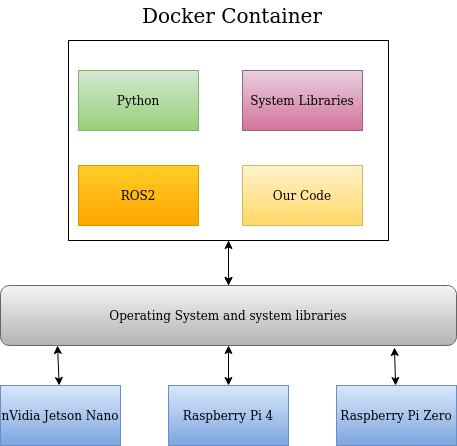
\includegraphics[scale=0.5]{fig/osdiag.png}
    \caption{Proposed Operating System Configuration}
    \label{fig:operating_system_proposed}
\end{figure}

In order to efficiently run the necessary software, we required a system configuration with robust hardware support. This system had to be compatible with a variety of Raspberry Pi hardware and the nVidia Jetson Nano. We decided to utilize the Python interpreted language for rapid prototyping. For the middleware and communication layer, we chose ROS2. \\

\textbf{ROS2 Introduction and Rationale}

Our first four proposals outlined in Section \ref{fig:architecture} each offer a certain degree of distribution. Distributing data processing across multiple hardware units necessitates machine-to-machine communication, a task for which the client specifically requested the use of ROS2. ROS2 is a comprehensive software suite designed for robotics, with its core feature being inter-process communication. By creating and building our software as ROS2 nodes, we can avoid dealing with networking complexities, as ROS2 abstracts them. In ROS2, nodes constitute a graph where edges represent topics. Nodes can publish and subscribe to these topics.\\

%Our first four initial proposals in \ref{fig:architecture} are all distributed to a degree. Distributing the data processing across multiple hardware units requires machine-to-machine communication. The client requested the use of ROS2 for this task. ROS2 is a software suite for robotics and its core feature is inter-process communication. By developing and building our software as ROS2 nodes we don’t have to deal with networking as this is abstracted away by ROS2. Nodes in ROS2 make up a graph where the edges represent topics. A node can publish and subscribe to topics.\\

\begin{figure}[H]
    \centering
    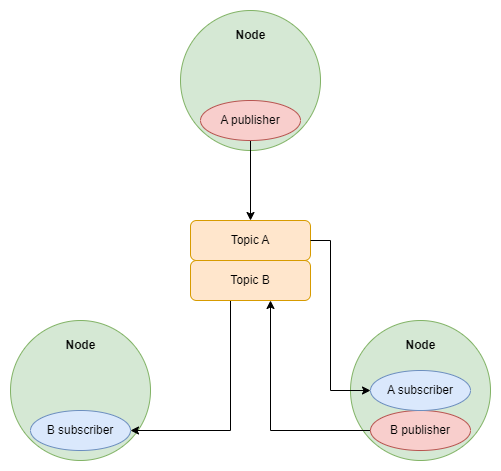
\includegraphics[scale=0.5]{a_martinbilder/ros_graph_example.png}
    \caption{Example ROS2 graph}
    \label{fig:ros_graph_example}
\end{figure}
Figure \ref{fig:ros_graph_example} presents a potential configuration of a ROS2 graph featuring three nodes. Beyond managing low-level communication between hardware units, integrating ROS2 contributes to high modularity, fostering the possibility for significant scalability. Upon reviewing our initial configurations, our client voiced interest in incorporating an additional single-board computer to further distribute the workload. This hardware expansion could also be implemented at subsequent stages without necessitating code rewrites. Essentially, nodes can be easily transferred from one hardware unit to another.\\

%Figure \ref{fig:ros_graph_example} illustrates how a ROS2 graph could look with three nodes. In addition to handling the low-level communication between hardware units, a ROS2 integration provides high modularity which creates a potential for high scalability. When proposed with our initial configurations, our client expressed their interest in adding an additional single board computer to further split up the workload. Adding hardware like this could also be done at later stages without rewriting any code. Nodes can simply be moved from one hardware unit to another.\\
\newpage

Our objective was to make an informed decision, ensuring we did not default to conventional software without considering potential alternatives that might offer performance benefits or simplified software deployment. Both the Raspberry Pi variants and the Jetson Nano are compatible with the Linux operating system. Linux, a free and open-source operating system, is available in several versions, commonly referred to as distributions or "distros". These distributions can greatly vary in terms of software availability and hardware support, contingent on the installed version. Consequently, we aimed to investigate the potential differences between these versions to determine which one best met our needs.

However, with over 600 distinct Linux distributions available, it was not feasible to evaluate all of them within our limited timeframe. To streamline our focus, we decided to sample the most commonly used distributions that also maintain an enterprise presence. Ultimately, we chose to evaluate Raspberry Pi OS, the version bundled with Raspberry Pi variants, along with Fedora Linux, openSUSE Linux, and Ubuntu.\cite{linuxcounter} \\ 

\newpage

After finalizing our decision, we turned our attention to designing our architecture, considering how the software would function on different hardware configurations and how we could ensure a uniform configuration across all systems. To this end, we explored the feasibility of running the software within what is commonly known as a container. A container is a compact, standalone, and executable software package that encompasses everything required to execute a piece of software, including the code, runtime, system tools, system libraries, and settings. Containers are isolated from each other and bundle their own software, libraries, and configuration files, communicating through well-defined channels. Implementing this technology would guarantee identical deployment configurations and could help mitigate any potential performance artifacts. The goal of this configuration was to encapsulate the necessary environment and libraries for ROS2 within these containers, as illustrated in Figure \ref{fig:dockerarch}.\\

\begin{figure}[H]
    \centering
    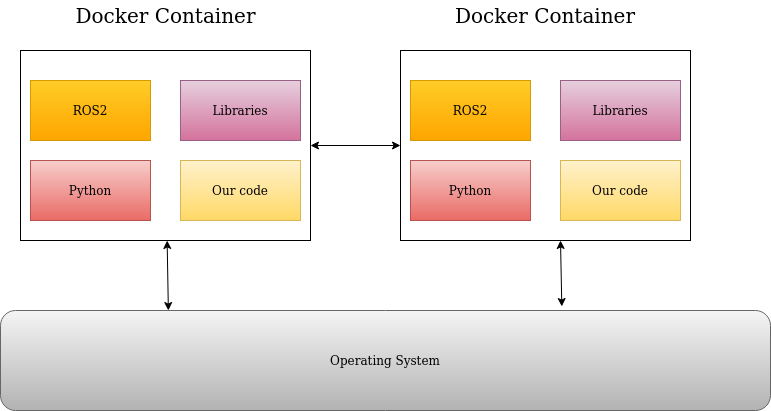
\includegraphics[scale=0.5]{fig/Docker Architecture.drawio.png}
    \caption{Docker architecture}
    \label{fig:dockerarch}
\end{figure}

Upon deciding which configurations to investigate, we initiated our examination by methodically installing the different distributions on physical hardware and assessing their functional capabilities and any shortcomings. As illustrated in Figure \ref{fig:osarch}, you can observe the different outcomes and ascertain which functions were successful and which were not. \\ 

\begin{figure}[H]
    \centering
    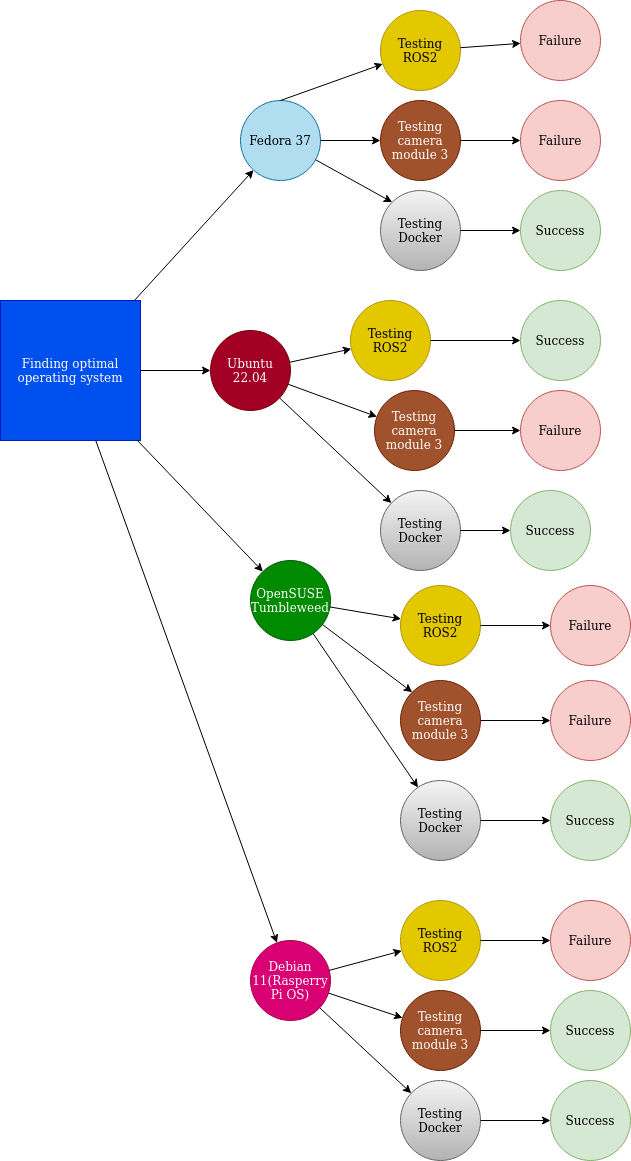
\includegraphics[scale=0.5]{fig/decision_os.png}
    \caption{Decision Process OS}
    \label{fig:osarch}
\end{figure}

\clearpage

As indicated in figure \ref{fig:osarch}, there were no systems that met all the requirements we had for our software platform, this caused a need to do further research in order to be able to decide which platform we would use going forward. \\

We further refined our choices to Ubuntu and Debian, as these platforms had only a single missing dependency. However, we needed to ascertain which option would offer the best outcomes relative to the efforts required to rectify each system.\\

\begin{figure}[H]
\centering
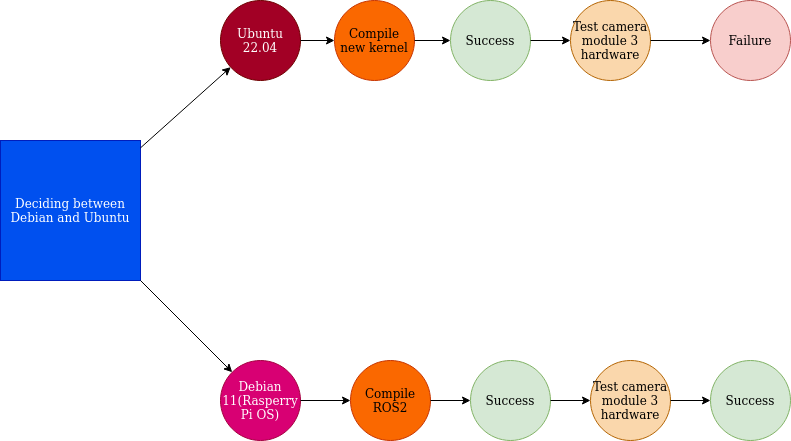
\includegraphics[scale=0.5]{fig/select_dist.png}
\caption{Decision Process Distribution}
\label{fig:distselect}
\end{figure}

Debian faced the disadvantage of having difficulties with the ROS2 operation, which entails a relatively complex and comprehensive build-system. The documentation can often be outdated due to the fast-paced advancement of the ROS2 project at the current stage. Conversely, Ubuntu's challenge lay in the lack of driver software for the Camera Module Version 3.\\

Given our limited experience with the ROS2 build system and the scant documentation on manual software building and installation, we decided to attempt installing the existing Debian driver in an Ubuntu environment. This would enable us to operate ROS2 with Camera Version 3.\\

\newpage

In the Linux operating system, drivers are typically formulated as modules and integrated with the operating system kernel. This kernel is the software component within an operating system that manages hardware resources. Within the Linux system, it is feasible to specifically compile this component for the running system, without interfering with the other system software components.\\

Our next step was to clone the git repository of the Raspberry Pi Foundation, given that the operating system bundled with these single-board computers (SBCs) supports that particular camera. Once completed, we managed to compile the Raspberry Pi OS kernel for our active version of Ubuntu.\\

After finalizing the installation and booting our new kernel, the hardware was detected, but there was no video output. At this juncture, we believed that we could get the hardware to function under Ubuntu, considering this as our best immediate course of action.\\

We proceeded with various tests under different configurations and compiled different versions of the Linux kernel, including an unmodified version directly from \url{https://kernel.org}. When none of these strategies produced the desired results, we were compelled to reassess our approach.\\

Our focus then transitioned towards an attempt at compiling ROS2 for Debian. We delved into the documentation to compile the software on our system. However, this task proved challenging, and we faced several hurdles while attempting to compile the software. As a temporary solution, we found someone who had compiled a Debian package on GitHub, albeit from an older build. We could not verify its applicability to our requirements, thus leaving us with necessary steps to continue deploying ROS2 while we concurrently operated an unsecured ROS2 installation, aiming to expedite development.\\

Following an extended period of continuous effort, we managed to compile ROS2 under a Debian system. This development allowed us access to Camera Module 3 and ROS2 on the same computer. The subsequent step involved deploying this to a Docker image, facilitating environment control and ensuring a consistent platform for our ROS2 source code.\\

However, an unfortunate consequence of compiling software is its substantial size growth. Post-building our Docker system, its size ballooned to 14GB, which was unwieldy for deployment and challenging to run on the Raspberry Pi Zero. Unfortunately, we were unable to rectify this issue in time for our project delivery. Although it does operate on the Raspberry Pi Zero, deployment is slow and can potentially create problems if the Zero exhausts memory while pulling the Docker image.\\

\subsection{Raspberry Pi 4 and Zero 2}
After reviewing our results from the selection process, we arrived at a proposed solution for our configurations based on the Raspberry Pi hardware and the Raspberry Pi OS. This solution mirrored the one depicted in figure \ref{fig:dockerarch}, thereby aligning closely with our initial research and concept.\\

\subsection{Jetson Nano System Software Configuration}

Upon finalizing the configuration for the Raspberry Pi, we shifted our focus to the Jetson Nano. Our initial plan was to have identical configurations across all hardware. However, the proprietary nature of Nvidia's hardware precluded the support of the Raspberry Pi OS.
This necessitated exploratory research on compatible software for the Jetson Nano, which would align closely with the Raspberry Pi configurations. We direct your attention to figure \ref{fig:jetsonnanodesc}, depicting the versions we attempted to install and set up on the hardware.\\

\begin{figure}[H]
    \centering
    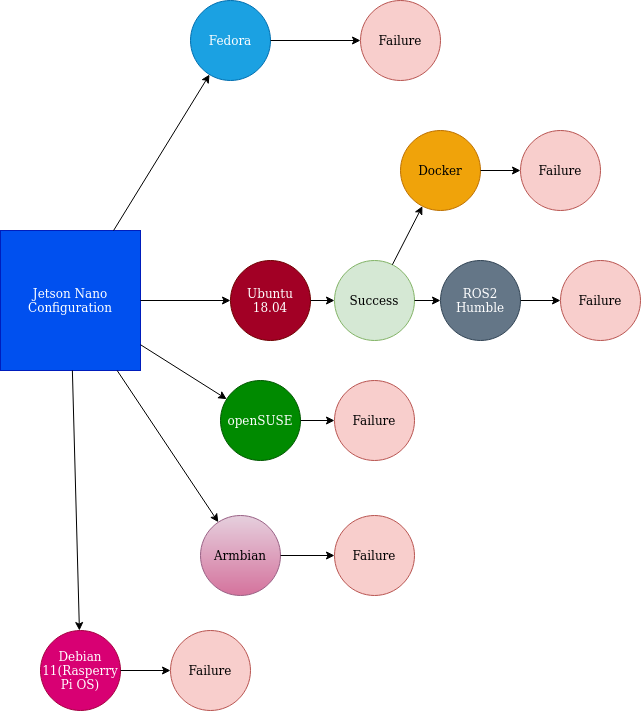
\includegraphics[scale=0.5]{fig/jetson_nano_os.png}
    \caption{Jetson Nano Decision Map}
    \label{fig:jetsonnanodesc}
\end{figure}

Following a rigorous testing phase where we attempted to run several different distributions on the Nano, we concluded that this approach was not an efficient use of our time. We chose instead to focus on executing the docker architecture on the bundled Ubuntu version running on the Jetson Nano. The supported version was released in April 2018. Despite its age, we believed that since Docker was available for it, we could adjust our container setup to secure a controlled environment to the extent possible.\\

\textbf{Docker Environment Jetson Nano}

When considering Docker on the Nano, we decided to implement the same configuration we had functioning on the other systems. However, adapting this to the hardware and software on the Nano proved challenging. Nvidia distributes the necessary software for the Nano in packages referred to as "Jetpacks". These packages are designed for use on specific versions of Linux that they ship with Jetson Nano; our version of the Jetson Nano was supported on Ubuntu 18.04, a five-year-old distribution. This presented challenges due to the rapid pace of change in many of the frameworks and Python libraries we wanted to use. Similar factors were also present in terms of features and performance improvements in the operating system itself.\\

Creating a Docker environment where we pass the GPU and every required library into the container in a functional manner proved to be a complex task. It demanded more expertise and time than we could provide during our project. Ultimately, the challenges posed by the Jetson Nano forced us to reconsider our architectural idea.\\

The final result for our Jetson Nano was that we utilized the system software bundled with the hardware, specifically Ubuntu 18.04. Owing to issues with Docker, we ran the software on the bare metal, as illustrated in figure \ref{fig:jetsonnanoros}. Moreover, unlike the Raspberry Pi configurations running ROS2 Humble, the Nano operates ROS2 Dashing. Despite these differences, the ROS2 architecture remains identical to the other configurations.\\

\begin{figure}[H]
    \centering
    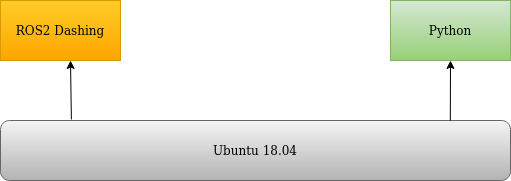
\includegraphics[scale=0.35]{fig/jetsonros.drawio.png}
    \caption{End Result Jetson Nano Architecture}
    \label{fig:jetsonnanoros}
\end{figure}
\newpage

\subsection{32-bit vs. 64-bit}
As Raspberry Pi OS 64-bit beats 32-bit in almost every metric regarding computation time \cite{32-bit_vs_64-bit} we decided to omit 32-bit based operating systems as a contender from this project.

\section{Proposed architectures}
\subsection{Initial Proposal}

Before we could start implementing our specific designs we needed to get the go-ahead from our client. We made a design sketch with five different configurations and presented these in order to reach an agreement on which areas we should focus on.

\begin{figure}[!h]
    \centering
    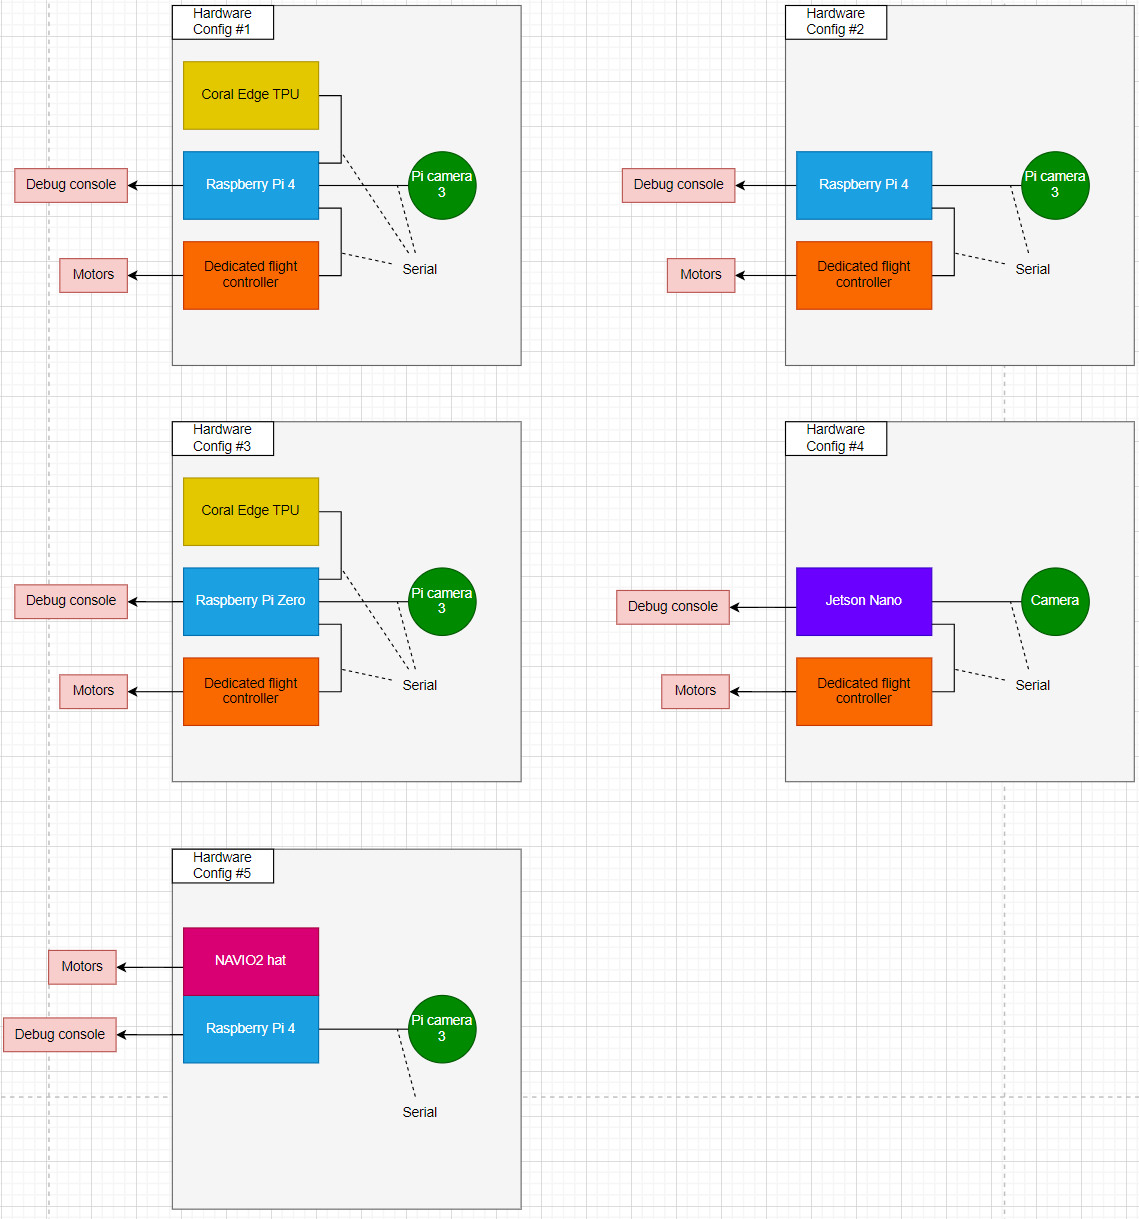
\includegraphics[scale=0.35]{fig/arkitektur.png}
    \caption{Initial architecture design}
    \label{fig:architecture}
\end{figure}
\newpage

From the figure \ref{fig:architecture} in this figure, you can see the five proposals which we presented to the client. These proposals were based on a variety of hardware configurations we had briefly discussed during meetings and the ones that we thought were the most likely to achieve our client's goals and deliver results that would show that this idea was viable. \\

\subsection{Second proposal}


\begin{figure}[H]
    \centering
    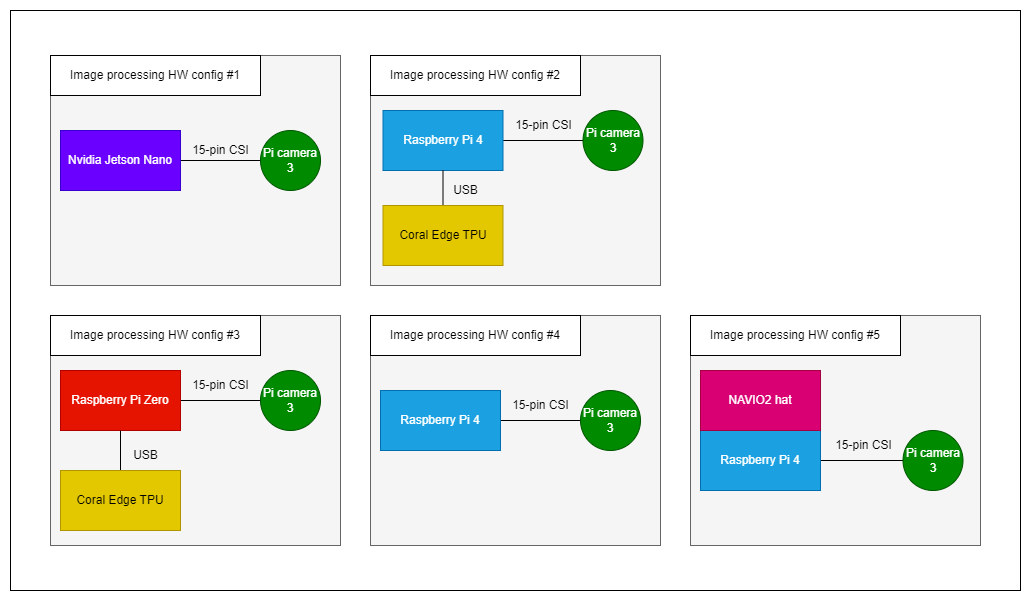
\includegraphics[scale=0.5]{a_martinbilder/hw_proposal2.drawio.png}
    \caption{Image processing modules}
    \label{fig:image_processing_prop2}
\end{figure}

\begin{figure}[H]
    \centering
    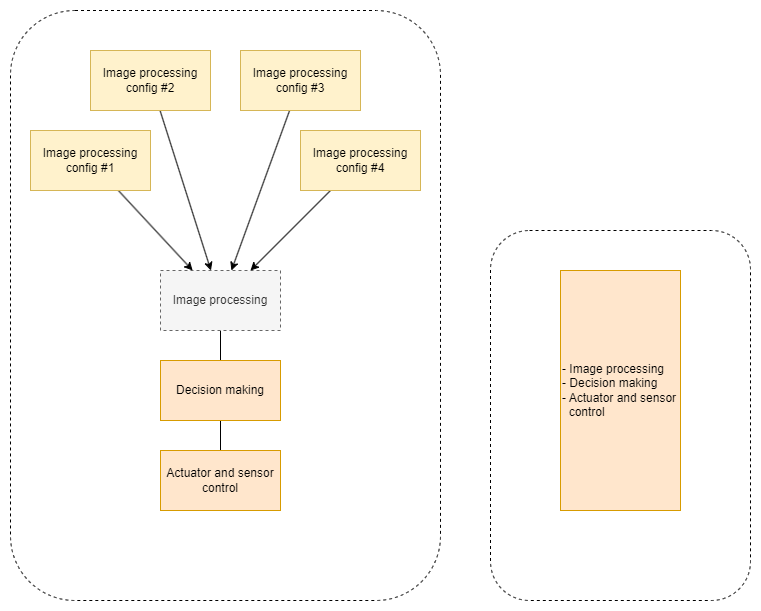
\includegraphics[scale=0.5]{fig/DistributedVsCentralized.png}
    \caption{Four distributed and one centralized architecture}
    \label{fig:distributed_vs_centralized}
\end{figure}

Figures \ref{fig:image_processing_prop2} and \ref{fig:distributed_vs_centralized} describe the second iteration of our hardware configuration designs. Our image processing hardware is now drawn as interchangeable modules, which plug into the rest of the drone. The “Decision making” module in \ref{fig:distributed_vs_centralized} represents a new single board computer, and the “Actuator and sensor control” module is the flight controller.
After further discussing our proposals with the client we agreed to drop configuration 5 due to time constraints. Discarding the centralized configuration gave us more time to explore image processing software, which at this point seemed to be the most time-consuming task ahead.\\

\subsection{Accepted architectures}
\label{sub:accepted_architectures}

Figure \ref{fig:accepted_hw_architectures} illustrates the final hardware architectures which were accepted by the client.

\begin{figure}[H]
    \centering
    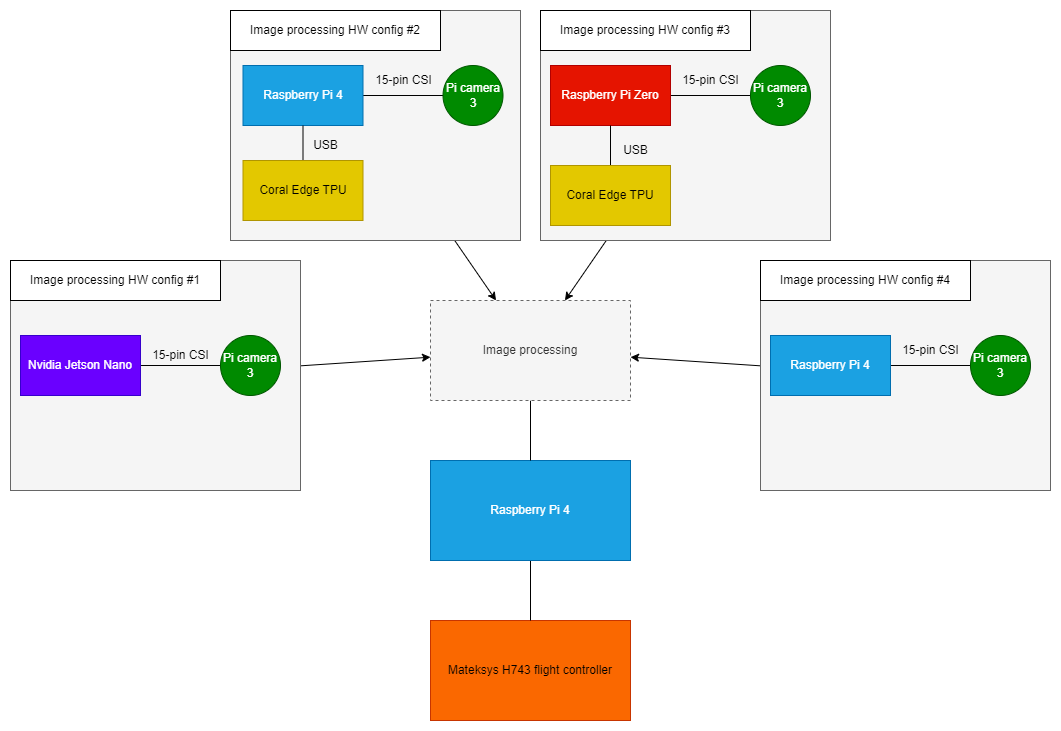
\includegraphics[scale=0.45]{a_martinbilder/accepted_hw_architecture.png}
    \caption{Hardware architectures accepted by client}
    \label{fig:accepted_hw_architectures}
\end{figure}


At this stage we had designed a high-level software architecture which shows our planned ROS2 nodes and how they should interface with each other. The architecture shown in figure \ref{fig:initial_software_architecture} is common for all our configurations. We decided that all 4 image processing modules should output the estimated distance to a detected object, and the detected object’s X and Y coordinates within the image frame. As a demonstration of a use case which needs the distance and position data, we designed the software architecture with “object following” in mind. For this use case the “Follow algorithm” node in figure \ref{fig:initial_software_architecture} would be a regulator which decides how the UAV should move to follow the detected object.

\begin{figure}[H]
    \centering
    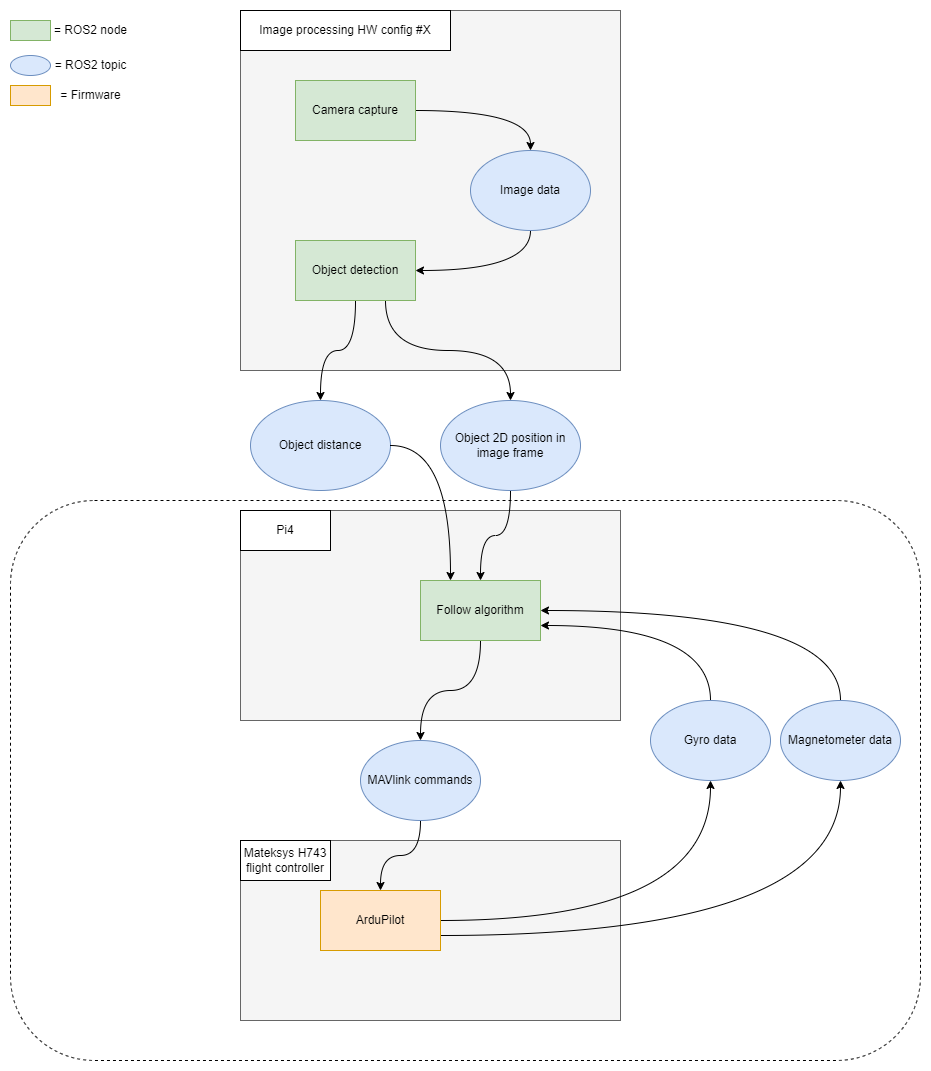
\includegraphics[scale=0.5]{a_martinbilder/initial_software_arch.drawio.png}
    \caption{Initial software architecture design}
    \label{fig:initial_software_architecture}
\end{figure}



\section{Object detection software}

One of the object detection systems we wanted to use was YOLO.\\

The YOLO (You Only Look Once) framework, developed by Joseph Redmon, revolutionized the field of object detection by providing a real-time object detection system. Contrary to traditional two-step object detection methods, where one step is dedicated to proposing regions where objects might exist and the second to classifying those regions, YOLO performs both tasks in one step. This makes it significantly faster and more efficient, which is particularly beneficial for applications that require real-time detection.\cite{YOLO}

The architecture of YOLO involves dividing the input image into a grid. Each grid cell predicts a certain number of bounding boxes and class probabilities. During the detection phase, bounding boxes with class probabilities below a certain threshold are discarded.

YOLO has gone through several iterations to improve its performance, in this study we have looked at YOLOv5 (released June 25th, 2020) \cite{YOLOv5}, and the latest YOLOv8 (released January 10th, 2023)\cite{YOLOv8}, both released by Ultralytics.

Given the novelty of YOLOv8, there was a lack of documentation regarding its operation on a Jetson Nano. All the available information concerning YOLO's operation on a Jetson Nano pertained to YOLOv5. Therefore, after meticulous comparison and deliberation, the decision was made to transition to the earlier iteration, YOLOv5.

Despite the commendable efforts of Ultralytics to simplify the application of YOLO, mastering the process of training on our own dataset, and effectively utilizing the diverse set of tools that accompany the framework, demanded a considerable investment of time. This learning curve demonstrates the complexity inherent in working with such advanced object detection systems. Readers are referred to the \ref{appendix:Yolo Training Tutorial} appendix for a concise guide on how to train models with custom data. Additional information and comprehensive documentation can be found on the Ultralytics website.

\subsubsection{Dataset}

In this study we decided on a common dataset for all the object detection models to be trained on. The dataset is divided into three distinct subsets - training, validation, and testing sets - each consisting of 110, 32, and 30 images respectively. The training set is used during the learning process, the model is then validated on the validation set at the end of each epoch. The test set is a dataset never seen before by the model and is used to do a final validation of the model.
Since we wanted to have a comparison between object detection and blob detection, we decided on a green tennis ball being the target for our models as this is easier to capture with blob detection.  


\section{Distance Measurement}

After wishes from our client, we've included the capability to calculate the distance to a detected object in our project. This is especially useful when considering the drone's relative position to the object and is particularly relevant for use cases such as landing. Understanding this distance becomes a key factor in ensuring precise and controlled landing maneuvers. \\

Due to the fact that we are using one singular camera, there is a problem getting the proper depth. The method we chose to use involves the idea of similar triangles to calculate the distance between a camera and an object. This method is based on the principle that the ratio of the object's actual width to its distance from the camera matches the ratio of the object's perceived width in the captured image (in pixels) to the camera's focal length. \cite{distanceobject}

To illustrate this concept mathematically, we introduce two similar triangles:

\begin{itemize}
    \item The first triangle (Triangle A) is constructed with the vertices being the camera, the object, and a selected point on the camera's image plane.
    \item The second triangle (Triangle B) includes the camera, the image of the object as perceived by the camera, and the identical point on the image plane as used in Triangle A.
\end{itemize}

In this scenario, the parameters for the two triangles are defined as follows:

\begin{itemize}
    \item In Triangle A, the 'height' is the distance to the object (D) and the 'base' is the actual width of the object (W).
    \item In Triangle B, the 'height' represents the camera's focal length (F), and the 'base' signifies the apparent width of the object in the image (P, in pixels).
\end{itemize}

Since the two triangles are similar, the ratios of the corresponding sides are equal, resulting in the equation:

\begin{equation}
\frac{D}{W} = \frac{F}{P}
\end{equation}

Using this equation, we can derive any one of the variables given the other three. For instance, the focal length of the camera (F) can be calculated by rearranging the equation to:

\begin{equation}
F = \frac{P \times D}{W}
\end{equation}

Furthermore, if the object's position shifts, altering the apparent width in the captured image (P'), the same equation can be adapted to compute the new distance (D'):

\begin{equation}
D' = \frac{W \times F}{P'}
\end{equation}



\section{Proposed Operating System and System Configuration}

After a comprehensive evaluation of operating systems suitable for various hardware configurations, we concluded that the Raspberry Pi configurations would utilize the system software provided with the devices. This decision was informed by the superior hardware support and the system's ability to effectively run ROS2 as required.\\

Contrarily, the situation with the Jetson Nano was distinct. Given the limited time for an in-depth exploration of the software construction on this platform, we decided to adhere to the configuration supported by nVidia. The final proposed system can be seen in Figure \ref{fig:sysconf}.

\begin{figure}[H]
    \centering
    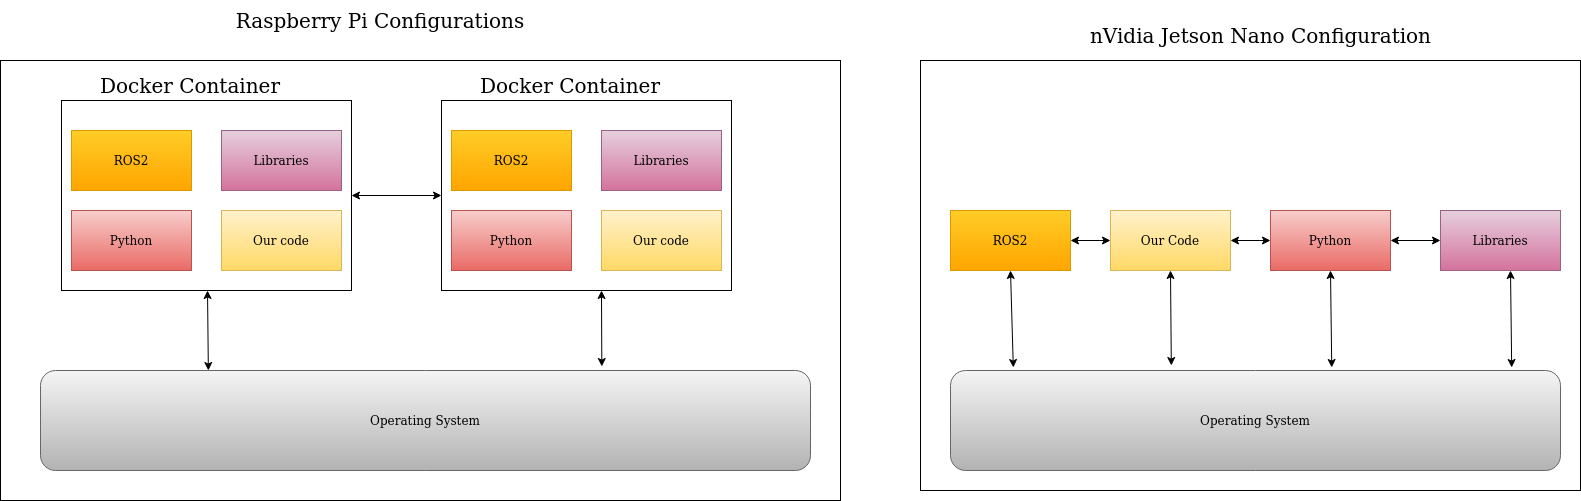
\includegraphics[scale=0.30]{fig/completeconfig.drawio.png}
    \caption{Finished Overview System Configuration}
    \label{fig:sysconf}
\end{figure}

\newpage

\section{Image processing modules}
In this chapter, we delve into the vital aspect of image processing configuration, a journey that has proven both challenging and enlightening. Our exploration began with an understanding of the integral role image processing plays in our project. As a technique that involves transforming or altering images using mathematical operations, image processing serves as a conduit that translates raw, visual data into a format that our systems can understand and utilize effectively.

Throughout this chapter, we discuss the myriad complexities involved in selecting, tuning, and applying appropriate image processing techniques and configurations. We recount our decision-making process, the technical considerations, the trial-and-error iterations, and the fortuitous insights that informed our eventual choices.

We acknowledge that the pathway toward effective image processing configuration is neither linear nor universally applicable. The optimal solutions often depend heavily on the specific contexts, goals, and constraints of the project at hand. However, we believe that by sharing our journey – our successes, our hurdles, and the lessons we learned along the way – we can provide valuable insights that may guide similar endeavors in the future.

Through this reflection, we aim to illuminate the depth and breadth of thought that underlies the seemingly mundane topic of image processing configuration, reinforcing its critical role in the success of our project and many others in the field. By the end of this chapter, readers will not only understand our journey toward an effective image processing configuration but also appreciate the intellectual richness that this journey entails.
\newpage

\subsection{Configuration 1, Jetson Nano}
This section aims to clarify the steps we followed to make object detection work on a Jetson Nano, incorporating details of unsuccessful attempts as well.

\begin{figure}[!h]
    \centering
    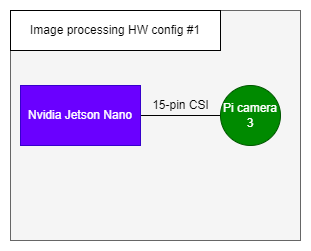
\includegraphics[scale=0.5]{fig/config1_hw.png}
    \caption{Hardware architecture, config 1}
    \label{fig:config1_hw}
\end{figure}


\subsubsection{Initial setup}

The NVIDIA Jetson Nano platform employs a software development kit (SDK) image known as JetPack, specifically version 4.6.1, which is the newest compatible version for the Jetson Nano device. JetPack 4.6.1 is built upon Ubuntu 18.04 (Bionic Beaver) and utilizes Python 3.6.9. The image is preconfigured with several essential developer tools, including TensorRT, cuDNN, and CUDA.\\

To flash the image onto the Jetson Nano, one can either use a terminal or the NVIDIA SDK Manager, which can be accessed at \cite{Jetson_sdk_manager}. It is strongly recommended to employ the NVIDIA SDK Manager for this task, as it significantly simplifies the installation process for the image and any additional SDKs. However, this method necessitates that the computer used for flashing possesses the same operating system as the target image. In the present case, the computer required reformatting to Ubuntu 18.04 to ensure compatibility.\\



Alternatively, the SD card can be directly flashed using the terminal. The necessary image can be obtained from the NVIDIA developer site \cite{Jetpack_461}. Subsequent instructions specific to your operating system can be found at \cite{Jetpack_461_write_to_sd}.\\

Following this, the NVIDIA SDK Manager can be used to install all additional SDKs via Secure Shell (SSH). This approach upholds the user-friendliness and efficient process inherent to the SDK Manager.

\subsubsection{Software overview}
Camera interface: Gstreamer and openCV\\
Object detector type: Deep neural network\\
Machine learning framework: Trained with Pytorch, TensorRT for inference\\
Model type: FP32 TensorRT model (.engine)\\
Model 1: 640x640x3 (Yolov5n)\\
Model output: Bounding boxes, prediction scores, class names, number of predictions\\
Model size: 7MB

\subsubsection{Config1 journey}


The process of getting infernece to run on the Jetson Nano platform has been a complex undertaking, with our efforts encompassing three distinct methodologies and two different models: MobileNet-SSD and YOLO. Each subsequent three subsection will delineate the specifics of these approaches. All methodologies employs TensorRT optimization to facilitate efficient execution on the NVIDIA hardware. The final method is the one currently in operation. see figure \ref{fig:storyline} for a visual representation of the journey.

\begin{figure}[H]
    \centering
    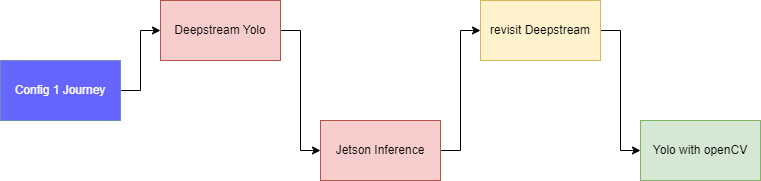
\includegraphics[scale=0.5]{evenbilder/storyline.drawio.png}
    \caption{Visual representation of the journey}
    \label{fig:storyline}
\end{figure}

\subsubsection{Yolo with Deepstream}
The process of deploying YOLOv5 on the Jetson Nano platform proved to be more complex compared to the implementation of MobileNet-SSD. The YOLOv5 documentation provides a dedicated page for its application on a Jetson Nano using a Software Development Kit (SDK) from Nvidia named Deepstream. However, the tutorial \cite{yolo_on_jetson}, last updated 18 November 2022) is not as straightforward as it might appear. For the purpose of this study, the deployment of YOLOv5 on the Jetson Nano was accomplished through two distinct approaches, both of which will be thoroughly explored in the following sections.


The initial step requires the use of a PC running Ubuntu 18.04 to operate the Nvidia SDK Manager in conjunction with the Jetson Nano. Following this, the installation of several additional packages, one of which is Deepstream, is necessary. This part of the procedure is fairly linear and should already be done with the initial setup of the Jetson.

The challenge arises when attempting to install dependencies for YOLO. Since YOLOv5 necessitates Python 3.7, while the Jetson Nano only supports Python 3.6.9, after cloning the repository, all entries in the requirements.txt file were commented out. Subsequent to numerous trials and errors, the tested system runs the following versions.

\begin{table}[H]
\centering
\begin{tabular}
{ |c|c| } 
\hline
Python package & Version number \\
\hline
gitpython & 3.1.20\\
\hline
matplotlib & 3.3.4 \\
\hline
numpy & 1.19.5 \\
\hline
opencv-python & 4.1.1\\
\hline
Pillow & 7.1.2\\
\hline
psutil & \\
\hline
PyYAML & 6.0\\
\hline
requests & 2.18.4\\
\hline
scipy & 1.5.4\\
\hline
thop & 0.1.1\\
\hline
tqdm & 4.64.1\\
\hline
seaborn & 0.11.0\\
\hline
setuptools & 59.6.0\\
\hline
\end{tabular}
\caption{pip packages used for deepstream}
\label{tab:yolo_requirements}
\end{table}
%gitpython>=3.1.20\\
%matplotlib>=3.3.4\\
%numpy>=1.19.5\\
%opencv-python>=4.1.1\\
%Pillow>=7.1.2\\
%psutil\\
%PyYAML>=6.0\\
%requests>=2.18.4\\
%scipy>=1.5.4\\
%thop>=0.1.1\\
%tqdm>=4.64.1\\
%seaborn>=0.11.0\\
%setuptools>=59.6.0\\


Continuing from this point, the subsequent steps as outlined on the GitHub repository should be followed until the DeepStream Configuration for YOLOv5 "Step 4. Generate the cfg and wts files". This can be accomplished with the following Python3 commands:

python3 gen\_wts\_yoloV5.py -w yolov5s.pt\\
python3 gen\_wts\_yoloV5.py -w custom.pt\\

Here, the user has the flexibility to either convert the pretrained yolov5s model or replace it with any model that has been subjected to transfer learning, as demonstrated above.

After completing the remaining steps, the user should be able to run inference on the included video. Additionally, to run inference on a Camera Serial Interface (CSI) camera, as employed in this study, the user must modify the source0 parameter in the deepstream\_app\_config.txt file as follows:



\begin{figure}[H]
    \centering
    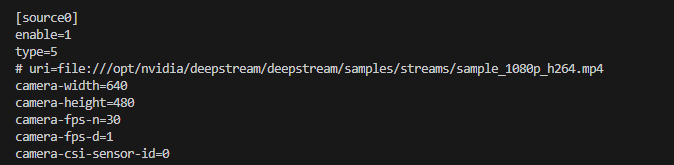
\includegraphics[scale=1]
    {evenbilder/yolo_deepstream_config.png}
    \caption{Deepstream app config file, source0}
    \label{yolo_deepstream_config}
\end{figure}

DeepStream offers built-in support for CSI cameras, with type=5 indicating the usage of a CSI camera. The camera's width and height can be adjusted according to the user's needs. It should be noted, however, that the model is optimized for an input resolution of 640x640 pixels, so providing an input close to this resolution would potentially enhance performance.\\

It is also important to modify the config-file under primary-gie, set this to config\_infer\_primary\_yoloV5.txt

To use a custom model, the configuration file must be modified in line with the particular version of YOLO in use, hence necessitating amendments to the 'config\_infer\_primary\_yoloV5.txt' file. The modifications include changes to the following parameters:

\begin{figure}[H]
    \centering
    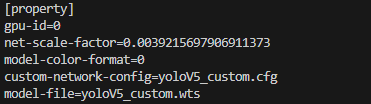
\includegraphics[scale=1]{evenbilder/yolo_deepstream__custom_model.png}
    \caption{config\_infer\_primary\_YoloV5.txt, custom model}
    \label{config_infer_primary}
\end{figure}

In this context, the weight (wts) and configuration (cfg) files have been renamed as 'yoloV5\_custom.cfg' and 'yoloV5\_custom.wts', respectively, indicating their customized nature and their association with the YOLOv5 model.
Now to run inference, simply use the command:\\
\\
deepstream-app -c deepstream\_app\_config.txt\\

As indicated on the Ultralytics webpage \cite{yolo_on_jetson}, the potential to achieve a rate of 30 frames per second (fps) exists when deploying a Jetson Xavier NX with FP32 and the YOLOv5s model. In contrast, the Jetson Nano, possessing lesser hardware capabilities than the Xavier, managed to reach a rate of 10 FPS with the YOLOv5n (Nano) model.

However, a substantial obstacle presented itself in the form of a 400 ms latency on the inference stream. Even with thorough system resource monitoring and various attempted solutions, the latency issue could not be mitigated. The implications of this problem suggested that the procedure overtaxed the Jetson Nano's hardware, thereby making it an unsuitable choice for applications like drone operations, which require instantaneous detection capabilities.

The Deepstream approach, despite its challenges, displayed a degree of adaptability. Specifically, it allowed a broad range of easy customizability via accessible configuration files.
\newpage



\subsubsection{Mobilenet-SSD}
Jetson Inference \cite{Jetson_inference}, a GitHub repository developed by Dustin Franklin from Nvidia, provides a well-documented tutorial complete with video walkthroughs, which is particularly beneficial for beginners in the field of computer vision working on the Jetson device. The process of getting this up and running is as simple as cloning the repo and then running the docker that is included. 

The pre-trained model demonstrated satisfactory performance at shorter distances but struggled with object detection when the objects were small or located at greater distances. To address this, transfer learning was applied to the model using our dataset, both on the Jetson device and on a separate computer equipped with a dedicated GPU. Despite training the model for over 1000 epochs, the inference failed to detect the object.

A survey of online forums confirmed that the model encountered difficulties with small objects. An attempt was made to upgrade the model to accommodate an input resolution of 512x512 instead of the standard 300x300. This was tried, and while this modification slightly improved the model's performance, it did not reach the level of the YOLO model trained earlier in the study. As a result, a decision was made to revisit YOLO.

\subsubsection{Yolo with openCV}

Since DeepStream did not yield satisfactory results, we searched for an alternative solution. During this exploration, we discovered newly created repository from Mailrocketsystems \url{https://github.com/mailrocketsystems/JetsonYolov5}. The repository applies TensorRT and OpenCV for inference. The configuration process is user-friendly, requiring merely adherence to the instructions provided in the repository's ReadMe file on GitHub.

The extraction of the right metadata from the model necessitates some modifications to the yoloDET script. Please refer to Figures \ref{fig:inference_before} and \ref{fig:inference_after} for the implemented changes.



\begin{figure}[H]
    \centering
    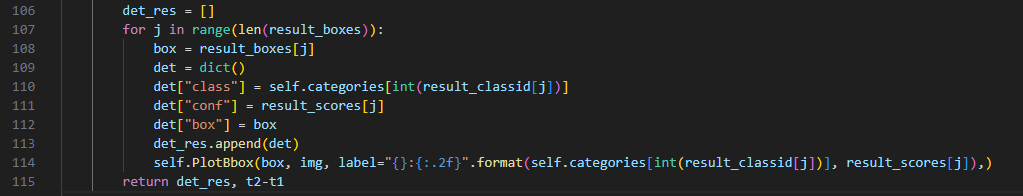
\includegraphics[scale=0.5]{evenbilder/yolo opencv/inference-before.png}
    \caption{YoloDET before}
    \label{fig:inference_before}
\end{figure}

\begin{figure}[H]
    \centering
    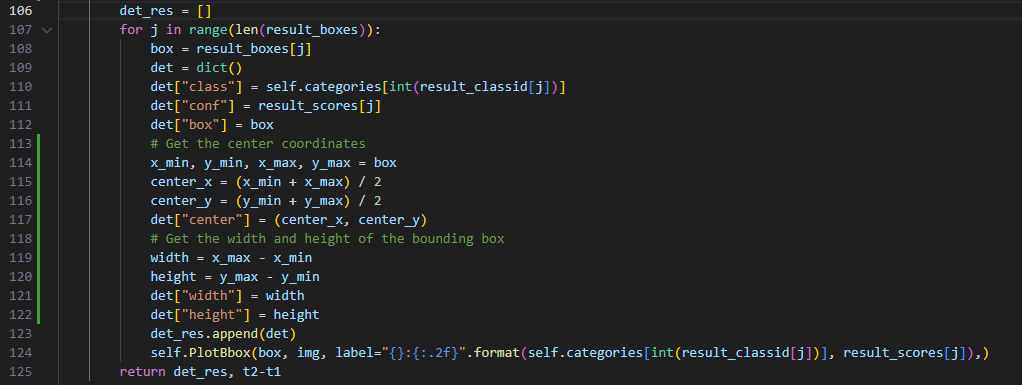
\includegraphics[scale=0.5]{evenbilder/yolo opencv/inference-after.png}
    \caption{YoloDET after}
    \label{fig:inference_after}
\end{figure}

Now we can simply edit the app.py script to use our model, and extract the metadata we just added in yoloDET. See figures \ref{fig:selecting_our_model}, \ref{fig:metadata_orginal}, \ref{fig:metadata_modified}\\

\begin{figure}[H]
    \centering
    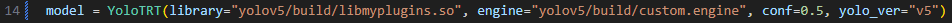
\includegraphics[scale=0.5]{evenbilder/yolo opencv/custommodel.png}
    \caption{Selecting our model}
    \label{fig:selecting_our_model}
\end{figure}

\begin{figure}[H]
    \centering
    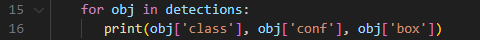
\includegraphics[scale=0.5]{evenbilder/yolo opencv/app1.png}
    \caption{extracting metadata original}
    \label{fig:metadata_orginal}
\end{figure}

\begin{figure}[H]
    \centering
    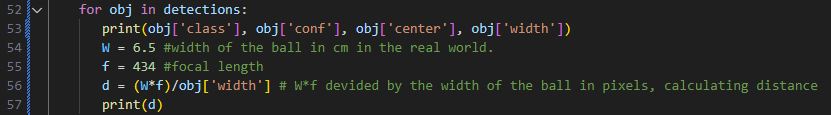
\includegraphics[scale=0.5]{evenbilder/yolo opencv/app2.png}
    \caption{extracting metadata modified}
    \label{fig:metadata_modified}
\end{figure}

The repository enabled us to perform inference in real-time with close no none latecy, which was particularly helpful in demonstrating the capabilities of the hardware within config1. 


\subsubsection{Reflections}


While the Jetson Nano boasts comparatively robust hardware, it is beginning to show signs of obsolescence, largely due to its reliance on an older version of the Jetpack SDK, which in turn is based on outdated versions of Ubuntu and Python. There have been considerable developments since Ubuntu 18.04 and Python 3.6. Nonetheless, we maintain that the Jetson Nano presents a compelling option for hobbyists seeking to delve into the realm of AI and explore its capabilities. For more advanced development pursuits, we would recommend a more contemporary model, such as the Jetson Orin Nano. This newer hardware is accompanied by support for the latest release of the Jetpack SDK, which is based on Ubuntu 20.04, and generally offers better compatibility with recent software.


The Jetson Nano was received quite late into the project, leaving us with approximately one month to set it up and get it working. With more time, and a deeper understanding of machine learning and ai, the results might have been different.


\newpage

\subsection{Configuration 2, Pi 4 w/ Coral Edge TPU}

\begin{figure}[h]
    \centering
    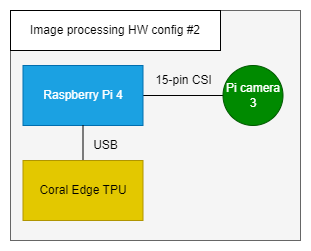
\includegraphics[scale=0.5]{fig/config2_hw.png}
    \caption{Hardware architecture, config 2}
    \label{fig:config2_hw}
\end{figure}


\subsubsection{Software overview}

\textbf{Camera interface:} picamera2 python library\\
\textbf{Object detector type:} Deep neural network\\
\textbf{Machine learning framework:} Tensorflow Lite\\
\textbf{Model type:} Tensorflow Lite model (.tflite) compiled for Coral Edge TPU\\
\textbf{Model 1 input:} 320x320x3 array (EfficientDet-lite0)\\
\textbf{Model 1 size:} 5.57MB (EfficientDet-lite0)\\
\textbf{Model 2 input:} 384x384x3 array (EfficientDet-lite1)\\
\textbf{Model 2 size:} 7.57MB (EfficientDet-lite1)\\
\textbf{Model outputs:} Bounding boxes, prediction scores, class names, number of predictions\\


\begin{table}[H]
\centering
\begin{tabular}
{ |c|c| } 
\hline
\textbf{Apt package name} & \textbf{Version} \\
\hline
python3-tflite-runtime & 2.5\\
\hline
python3-cv-bridge & 1.16.2\\
\hline
libedgetpu1-std & 16.0\\
\hline
python3-picamera2 & 0.3.9\\
\hline

\end{tabular}
\caption{Required apt packages, config 2}
\label{tab:config2_apt_packages}
\end{table}

\begin{table}[H]
\centering
\begin{tabular}
{ |c|c| } 
\hline
\textbf{Pip package name} & \textbf{Version} \\
\hline
numpy & 1.20\\
\hline
\end{tabular}
\caption{Required pip packages, config 2}
\label{tab:config2_pip_packages}
\end{table}


\subsubsection{Video capture software setup}

The configuration runs inference on image data provided by the Pi camera V2. The Picamera2 library is the Python interface to the currently supported Raspberry Pi camera stack. Picamera2 requires Raspberry Pi OS Bullseye or newer versions, and the legacy camera stack must be disabled through the raspi-config utility.\\

\subsubsection{Inference software setup}

Setting up the configuration with Python is straightforward as the Coral Edge TPU is well documented by Google’s Coral team. The TPU is only compatible with Tensorflow Lite models so the Tensorflow Lite Python API (Tensorflow Lite Runtime) is needed to run inference. Additionally, the Edge TPU runtime library is needed to provide an interface between Tensorflow Lite Runtime and the TPU. At the time of writing Tensorflow Lite Runtime is only compatible with Python versions 3.7 – 3.9.\\

\subsubsection{Deep learning models}

Using the same dataset as in configuration 1, we have trained 2 suitable models for this configuration. The models are trained with transfer learning on pre-trained neural networks. We used Tensorflow Lite Model Maker for training. This library simplifies transfer learning to a degree that allows it to be done with minimal knowledge of the inner workings of Tensorflow and neural networks. Using Tensorflow Lite Model Maker had the downside of limiting our options for pre-trained models. The library only supports 5 different object detection models, which are all from the EfficientDet family released in late 2019. We selected EfficientDet-lite0 and EfficientDet-lite1 for this configuration. These models are optimized for Tensorflow Lite and edge deployment \cite{efficientDetLite0} \cite{efficientDetLite1}. EfficientDet-lite0 is the lightest model with an input size of 320x320x3. EfficientDet-lite1 is slightly heavier with an input size of 384x384x3. An attempt was made to compile a custom Yolo v5 model for Tensorflow Lite and the Edge TPU for a better comparison against configuration 1. The Yolo model was discarded as we were unable to have it utilize the TPU. The Coral Edge TPU puts multiple constraints on the model choice \cite{edgetpuModels}, one of them being that not all commonly used neural network operations are supported. Deducing why our yolo model failed to run on the TPU was beyond the scope of this study, as it would likely require deep understanding of neural networks.\\

\subsubsection{Training the models}

We used transfer learning with the Tensorflow Lite Model Maker library to train models for configuration 2. We explored the possibility of using Keras as well, which is a high-level deep learning API with Tensorflow integration. Using Keras would enable us to use any available object detection model for transfer learning. While Model Maker only supports 5 object detectors. Model Maker was selected because of its low complexity. Due to our time constraints, we chose not to dedicate time to learning Keras.
Before training we prepared our dataset by annotating our images. The dataset used is the same as the one used in configuration 1.
The dataset is annotated using Labelimg, which is a GUI application for manually labeling objects. Labelimg generates an xml file for each image in the Pascal VOC annotation format. The annotation contains info on the bounding box location and class name for labeled objects in an image. Figure \ref{fig:pascalvoc} shows the content of an xml file, and its corresponding image with the bounding box drawn around our labeled object.

\begin{figure}[H]
    \centering
    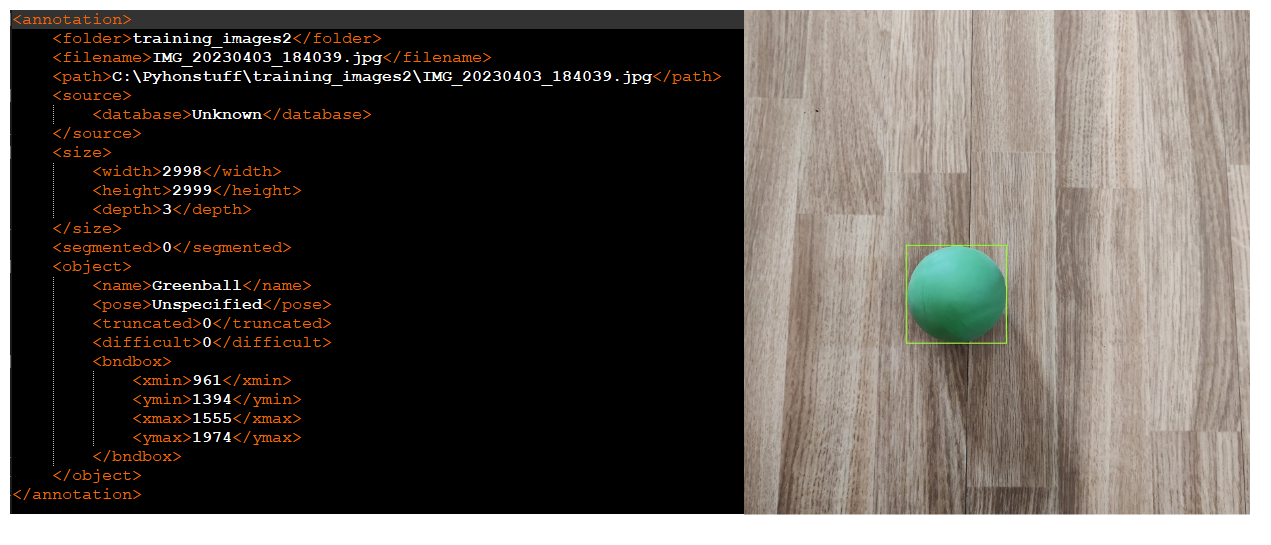
\includegraphics[scale=0.3]{a_martinbilder/pascalvoc_xml.drawio.png}
    \caption{Pascal VOC .xml contents (left), corresponding image (right)}
    \label{fig:pascalvoc}
\end{figure}

The annotated dataset is split into three categories: Training data, validation data and test data. Training data is the set used for training our model. The validation data is used to evaluate the model during the training process. Test data is used to evaluate the final model after training is complete. The final evaluation gives us the model’s precision statistics. The simplicity of Tensorflow Lite Model Maker is best described by the few lines of code required to train a model. Our training script for transfer learning with the EfficientDet Lite1 model can be found in \ref{appendix:ModelMaker}. When the Tensorflow Lite model is trained it needs to be compiled for the TPU. The compilation is done using the Edge TPU Compiler tool which can run on any Linux machine \cite{edgetpuCompiler}


\subsubsection{High level data flow}


Figure \ref{fig:config2_sw} shows the input and outputs of the Tensorflow Lite interpreter object which contains all the methods used to handle inference.
The picamera2 python library provides an interface to the Raspberry Pi camera drivers and allows us to capture image frames as multidimensional arrays. The tflite{\_}interpreter class provides methods for setting up and running inference with our trained object detection model. The model takes the image array as input and outputs the coordinates of bounding boxes around any detected object as well as a prediction score per detected object. The score describes how likely it is that the detection is a true positive. The full source code for configuration 2 can be found in appendix \ref{appendix:NodeCode}\\

\begin{figure}[H]
    \centering
    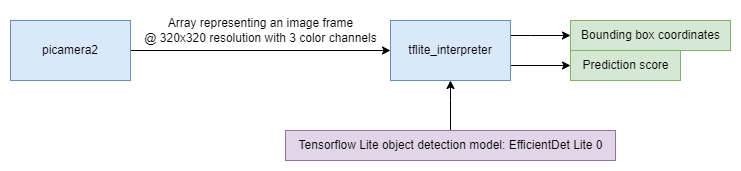
\includegraphics[scale=0.5]{fig/config_2_3_software_highlevel.drawio.png}
    \caption{Software, config 2}
    \label{fig:config2_sw}
\end{figure}

\subsubsection{Reflections}
This section covers aspects of configuration 3 we would have liked to explore further, if given the time.\\
\begin{itemize}
\item \textbf{Camera choice:} EfficientDet Lite 0 and 1 take input images in the sizes 320x320 and 384x384 respectively. Capturing video at resolutions above these values are a waste of resources. We should have used a camera with the ability to capture at low res with a high Field of View. Pi Camera V2 can capture at 640x480, but at this resolution the field of view is severely limited\cite{picameraFOV}. This issue could likely be resolved by using a different camera, unfortunately it was an issue we discovered very late in the project.
\item \textbf{Models:} Getting the YOLOv5 model used in configuration 1 to run on the TPU would result in a better comparison between the two.
\item \textbf{Multi TPU setup:} We only purchased one TPU which left us unable to explore the effects of a multi TPU setup. The Edge TPU Compiler can compile models in segments, each segment then runs on an individual TPU increasing the total throughput.
\end{itemize}




\subsection{Configuration 3, Pi Zero w/ Coral Edge TPU}

\begin{figure}[H]
    \centering
    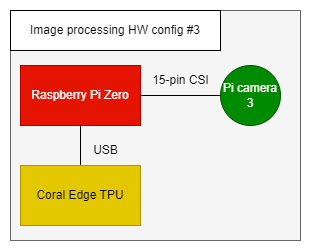
\includegraphics[scale=0.5]{fig/config3_hw.png}
    \caption{Hardware architecture, config 3}
    \label{fig:config3_hw}
\end{figure}

\subsubsection{Software}

Configuration 3 runs the same software as configuration 2.

\subsection{Configuration 4, Pi 4}

\begin{figure}[h]
    \centering
    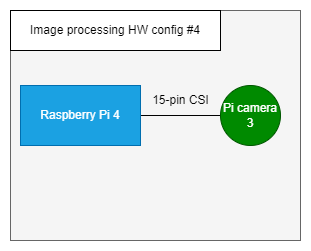
\includegraphics[scale=0.5]{fig/config4_hw.png}
    \caption{Hardware architecture, config 4}
    \label{fig:config4_hw}
\end{figure}

In this section, we will present Configuration 4, which stands out as the sole configuration that does not incorporate hardware acceleration, unlike the other configurations discussed in this report.

\subsubsection{Blob detection software}

For image capture, we use the Pi Camera V3, interfaced via the Picamera2 library. And for image processing, we implement OpenCV \cite{OpenCVDoc}, a widely-used library known for its powerful computer vision and image processing capabilities. It is particularly suitable for blob detection because of its versatility, efficiency, and ease of use. We also used a helper library, cvzone \cite{CVzoneDoc}, to reduce code and complexity. 

\subsubsection{Blob detection models and techniques}

We opted for blob detection or blob analysis \cite{OpenCVBlob}, an image processing technique that identifies and analyzes distinct areas of interest within an image. In the context of our project, blob detection was tasked with identifying balls of different colors.

Blob detection was chosen for its adaptability and precision. It can be finely tuned to detect specific objects, has a high degree of flexibility to meet different computational needs, and is particularly suited to the Raspberry Pi 4's limited processing power. These attributes made blob detection a compelling choice, as our project's aim was to balance detection accuracy with computational efficiency.

To identify the desired objects, our blob detection algorithm utilizes the HSV color space\cite{HSV}, which separates the hue, saturation, and value/brightness components of an image. By selecting appropriate color ranges, we are able to isolate specific objects based on their distinctive color properties.\cite{OpenCVBlob} Once we have found a colored object through color-based detection, our algorithm employs mathematical equations to analyze the contour properties of these objects. Specifically, we determine whether the contours of the detected blobs exhibit circular characteristics. This step helps differentiate the desired balls from other shapes or artifacts in the image. \cite{OpenCVContours}

Blob detection offers a high level of modifiability, allowing it to be tailored to meet specific computational requirements. By adjusting key parameters, the algorithm can be implemented with minimal computational resources, making it suitable for applications where processing power is limited. Alternatively, a larger set of parameters can be utilized, enabling more intricate analysis and detection of complex blobs. However, it should be noted that this approach requires higher computational resources. 

Considering the limitations of the Raspberry Pi 4 without acceleration hardware, the modifiability of blob detection allows us to strike a balance between detection accuracy and computational efficiency. We can optimize the algorithm by fine-tuning parameters to ensure reliable performance on this hardware platform. 

\subsubsection{Software overview}

Camera interface: Picamera2 Python library\\
Object detector type: Blob detection algorithm\\
Image processing library: OpenCV and cvzone\\
Model input: Images from Pi Camera V3\\
Model output: Coordinates of HSV color values and contour properties (circle)\\

OpenCV and our blob detection algorithm process these frames to identify distinct blobs (regions of interest) within the image. The algorithm outputs the coordinates of detected blobs, along with their HSV color values and contour properties. 

\subsubsection{Config4 journey}

\begin{figure}[H]
    \centering
    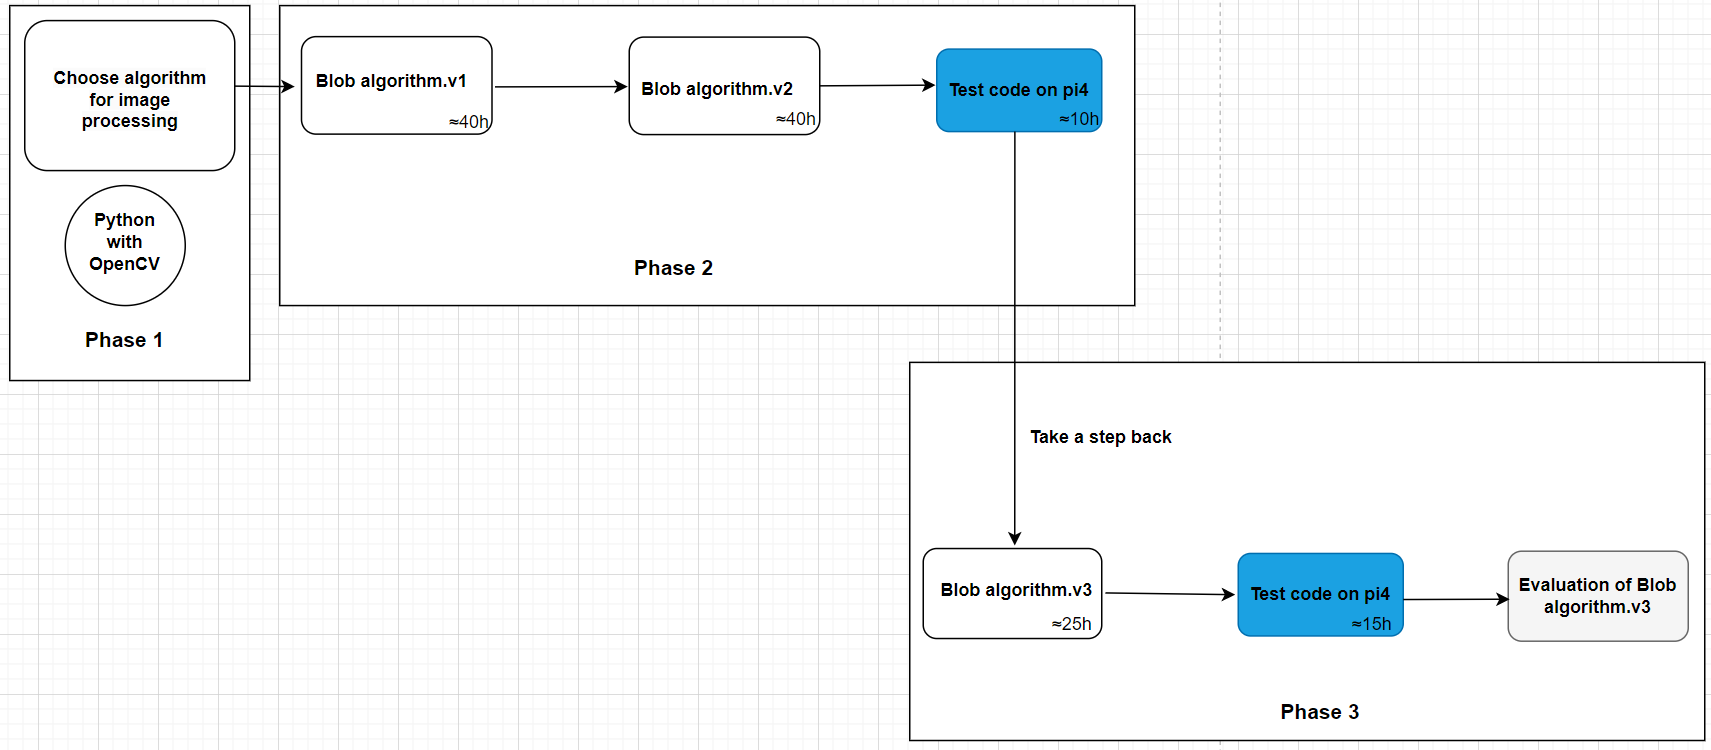
\includegraphics[scale=0.5]{fig/config4model.png}
    \caption{Config model, config 4}
    \label{fig:config4_model}
\end{figure}

To provide a clear and comprehensive understanding of our journey through this configuration, we developed a model accompanied by an explanatory guide. The model is divided into three phases, which illustrate the different stages of our work, the problems we encountered, and the solutions we implemented. This approach offers a better view of how our project developed from start to finish. 

In the first phase of our task, we decided to use Python with OpenCV for image processing. Python is a flexible and user-friendly language, making it an ideal choice for quick development. OpenCV is a powerful tool for image processing, offering a wide range of optimized algorithms. Using Python and OpenCV together enabled us to build and test our image-processing algorithms efficiently and effectively. 

After deciding to use Python and OpenCV for image processing, we needed to choose a suitable algorithm for our task. We selected blob detection, considering its efficiency and simplicity. This algorithm was an easy choice due to the lack of computing resources in our configuration. It’s important to note that efficiency and effectiveness can still depend on the specifics of a task. 

Moving to the second phase, we knew one of our client's wishes was for us to develop a program capable of detecting three tennis-sized balls, each of a different color. The program was also required to calculate and display their x, and y coordinates, the distance of each detected ball, and FPS on the frame. Initially, we worked in such a way that we developed and tested the program on a high-end laptop with a webcam. At this point, our blob detection algorithm could only detect the ball at approximately 1m, when our goal was to detect it up to 3-4m. Here is a picture of how we defined the color range for detection. 

\begin{figure}[H]
    \centering
    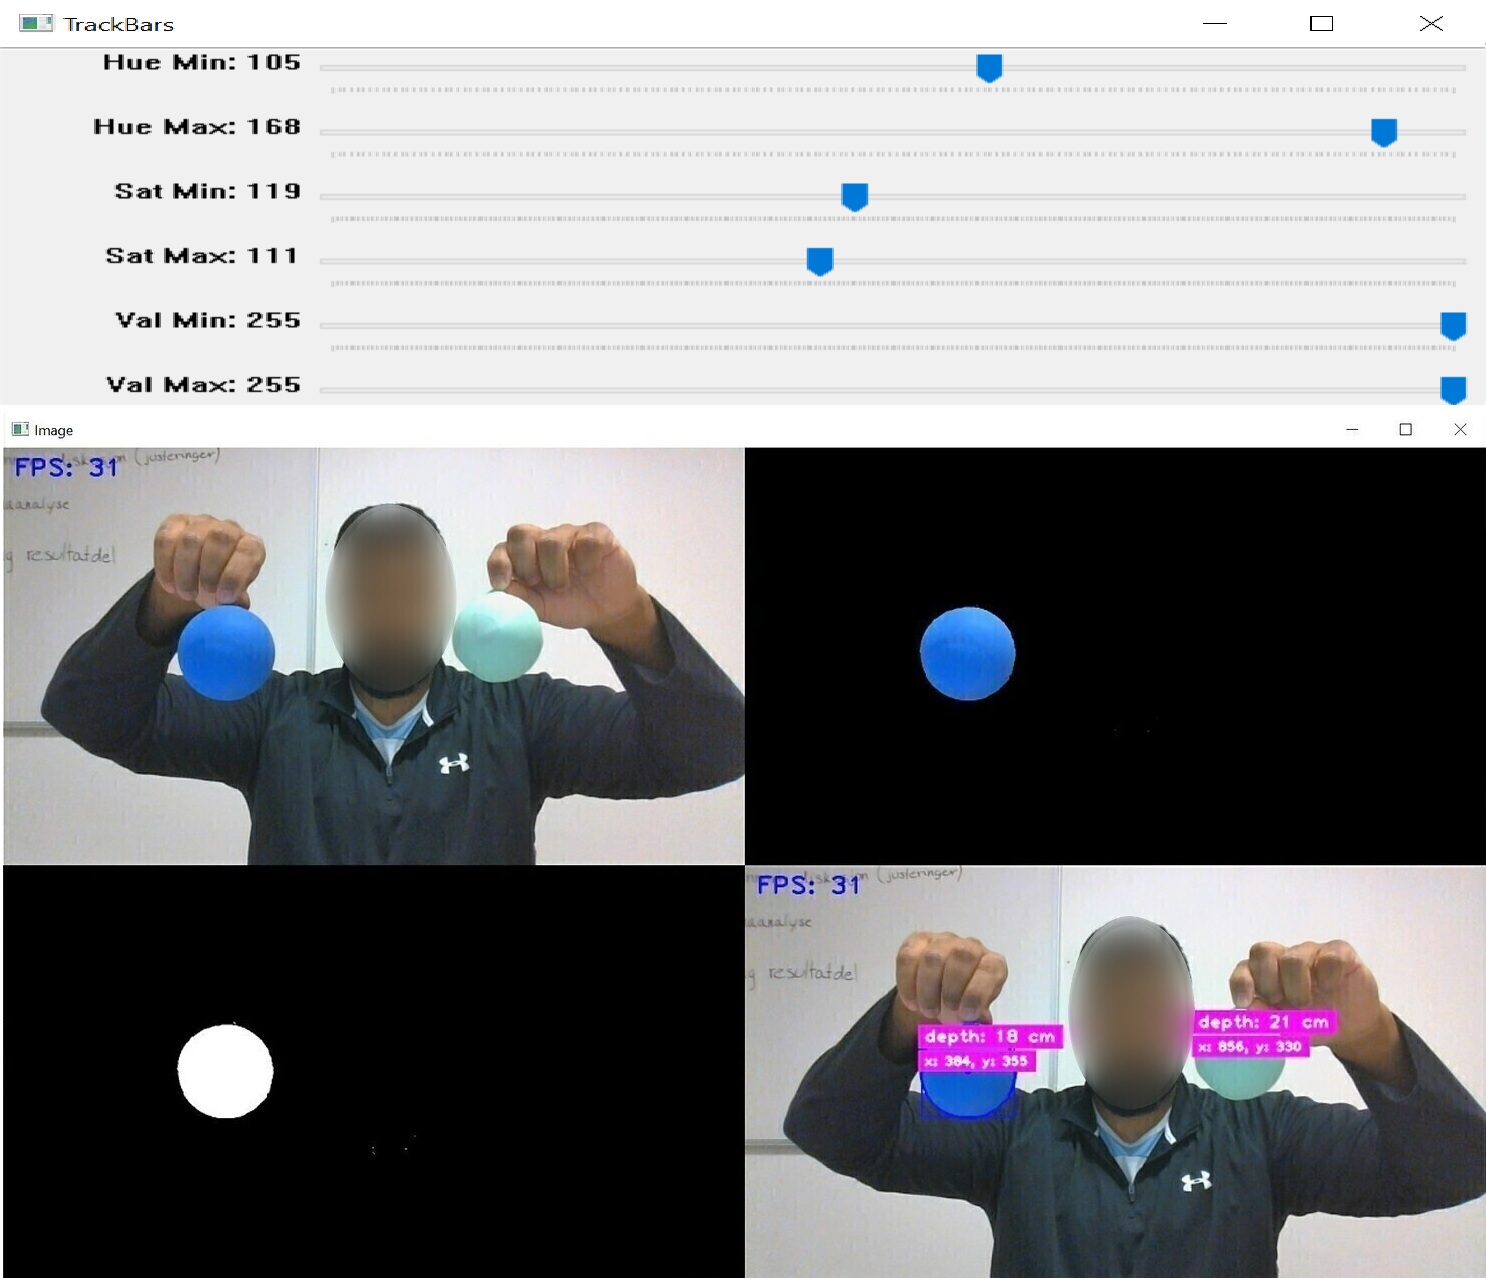
\includegraphics[scale=0.5]{fig/HsvColor.jpg}
    \caption{ColorFinder object, config 4}
    \label{fig:config4_color}
\end{figure}

Having realized that the initial version (Blob detection.v1) \ref{ch:algo} of our program did not fulfill the client's requirement, it became evident that we had to improve our blob detection. As we went to the next step to expand the program's capabilities from detecting one ball to three balls, the computational demands increased, which lead to the challenge of balancing efficiency and performance within our resource constraints.  

With the improvements in place, our v2 version \ref{ch:algo} of the program had advanced to the point where it could successfully detect three differently colored balls, simultaneously displaying their depth along with their x and y coordinates within the frame. However, despite better efficiency and accuracy, we were yet to reach our objective of detecting the balls from a distance of 3-4 meters. Furthermore, the frame rate was still a matter of concern, as we were only able to achieve an average of 4-8 frames per second, varying based on the resolution scale. 

\begin{figure}[H]
    \centering
    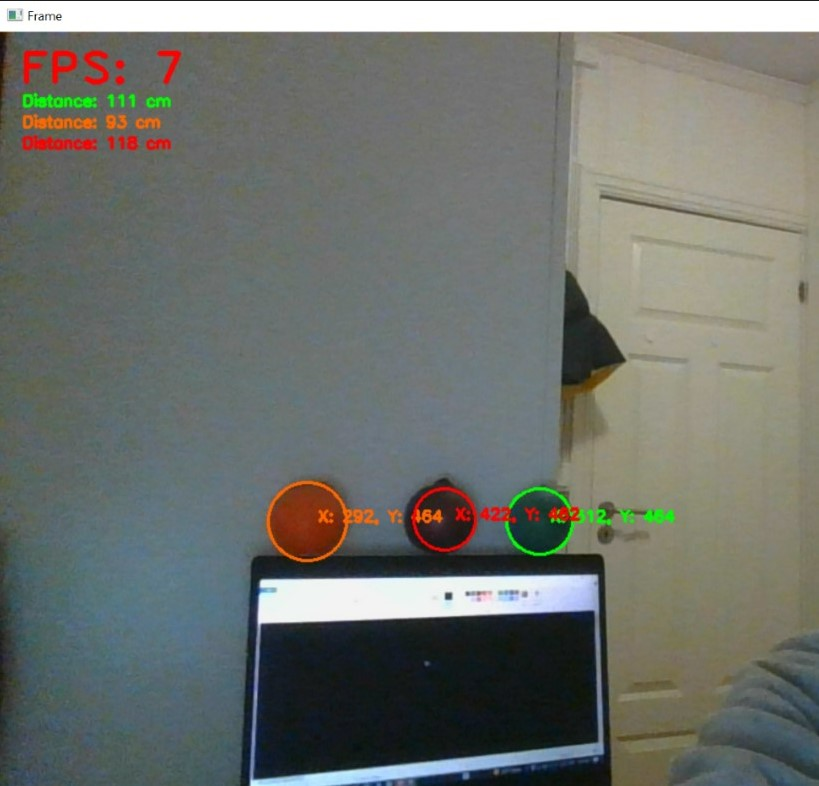
\includegraphics[scale=0.5]{fig/BlobDetection.v2.jpg}
    \caption{BlobDetection.v2, config 4}
    \label{fig:config4_v2}
\end{figure}

Upon testing the program on a Raspberry Pi, we found that the computational demands were too high for the hardware to handle effectively since we built and tested the program on a high-end laptop using the webcam.  As a result, we needed to revisit our approach and develop a more simplified version that could effectively run on the Raspberry Pi. 

In the third phase of our progress, in response to the computational constraints, we developed a simpler blob detection algorithm for the v3 version \ref{ch:algo}. By simplifying and removing some of the more computationally intense functionalities from the program, we were able to finally achieve the detection of the balls from a distance of 3-4 meters on our PC. While the precision of this version was somewhat compromised in comparison to v2, it was a necessary trade-off given our resource constraints. This version also offered a significant improvement in frame rate performance as we were now achieving between 20-25    frames per second, also resolving the previous frame rate issues we had encountered.

Upon testing our code on the Raspberry Pi, we encountered consistent results, primarily due to the frame rate on the desktop PC being limited to 30 fps. Due to the change of cameras being used from webcam to pi camera 3, the HSV values needed to be updated. The code can be modified to be more accurate with further iterations since we see that we can press the raspberry pi even further. 

To further test our configuration, we set out to evaluate the effectiveness of our blob detection. For this purpose, a script was developed to process labeled validation images, calculating precision, recall, and eventually yield the f1 score. This precision metric was chosen to compare our algorithm's performance with a trained model.

The optimal score we achieved was the result of testing over 10,000 different combinations of HSV values:

\begin{figure}[h!]
\centering
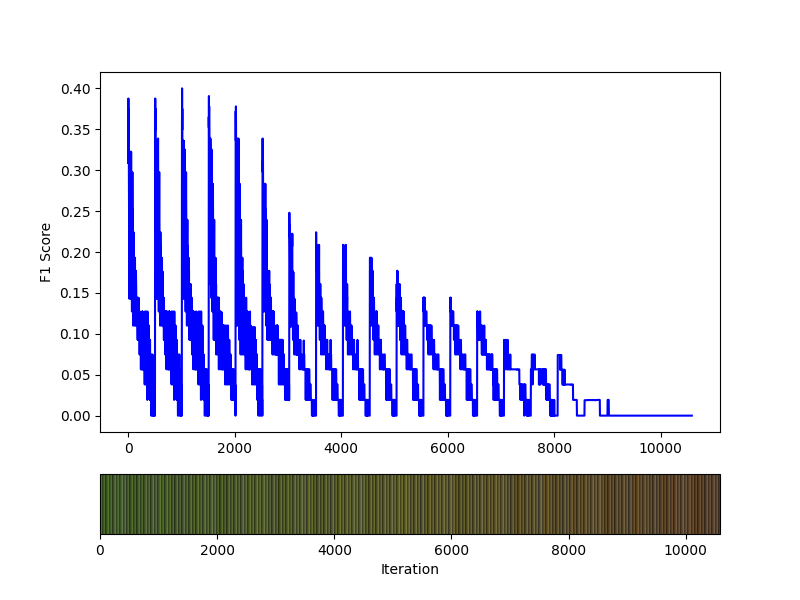
\includegraphics[scale=0.75]{sindrebilder/HSVfinal.png}
\caption{Trying different HSV combinations}
\label{fig:evaluationTest4}
\end{figure}

It's important to clarify that this figure does not aim to showcase the accuracy of our algorithm. Rather, it demonstrates our methodology for optimizing the F1 score across a set of images with varying lighting conditions and environmental factors. \ref{C4evaluation}

However, given the algorithm's dependency on HSV values, its performance varied significantly under different lighting conditions.\cite{Config4Dataset} This was a result of predetermined HSV values becoming inconsistent under varying lighting conditions, leading to inaccurate detections and incomplete detection of objects. To evaluate this, we utilized one image set captured under a wide variety of conditions. The images were taken in different environments, with lighting and distance variables changing extensively. The performance in these assorted conditions yielded varied results, indicating that the image set's robustness under uniform lighting conditions does not necessarily translate to the same level of accuracy under diverse lighting and environmental conditions.

The final test was done on FPS, where we recorded the fps over 30 secounds. This test was done using the ROS architectures and was relativly stable. We had one drop in FPS, but we did not have the time to investigate the manner further.

\subsubsection{Complexity}

While the initial implementation of the blob detection was relatively straightforward, achieving optimal performance was a more intricate process. It required meticulous fine-tuning of parameters to adapt to various conditions, and additional efforts were needed to handle the irregularities present in real-world data.

Maintenance added to the overall complexity, with a recurring need to manually adjust HSV values each time the environment changed. This repetitive process, although not adding significant complexity, was time-consuming and could potentially impact overall system efficiency. It's an area we aim to improve in future iterations of the project.

Despite these complexities, this configuration proved less complex in comparison to others, due largely to fewer encountered difficulties underway.



%\section{Technical overview}

%Our study aims to evaluate and compare four distinct distributed drone architectures, along with one centralized architecture. The distributed architectures solely vary in their approach to image processing. The leftmost diagram in figure \ref{fig:distributed_vs_centralized} illustrates a high-level overview of the four distributed architectures, wherein each box represents hardware with processing capabilities. The rightmost box represents the centralized architecture, where all the processing tasks are performed on a single hardware unit.

\section{Configurations, full context}

In this section, we present our configurations in the full UAV context, from image processing to the flight controller. We will cover ROS2 integration of the image processing modules, and the ROS2 nodes we have developed as we worked towards a complete UAV system.

\subsection{ROS2 integration}

As all image processing modules have the same outputs, the process of integrating them with ROS2 is the same for each module.
An image processing module is split into two nodes which each handle a specific task. One node handles video capture, while the other node handles object detection. The benefit of this modular approach is not obvious for our configurations as both video capture and object detection run on the same hardware. Having the option to run these nodes on dedicated hardware could be useful in the future, which is why we went with the modular approach. An abstract explanation of our nodes can be found in figure \ref{fig:node_description}. For more details see appendix \ref{appendix:NodeCode}, which contains commented code for each node we have developed.

\begin{figure}[h!]
    \centering
    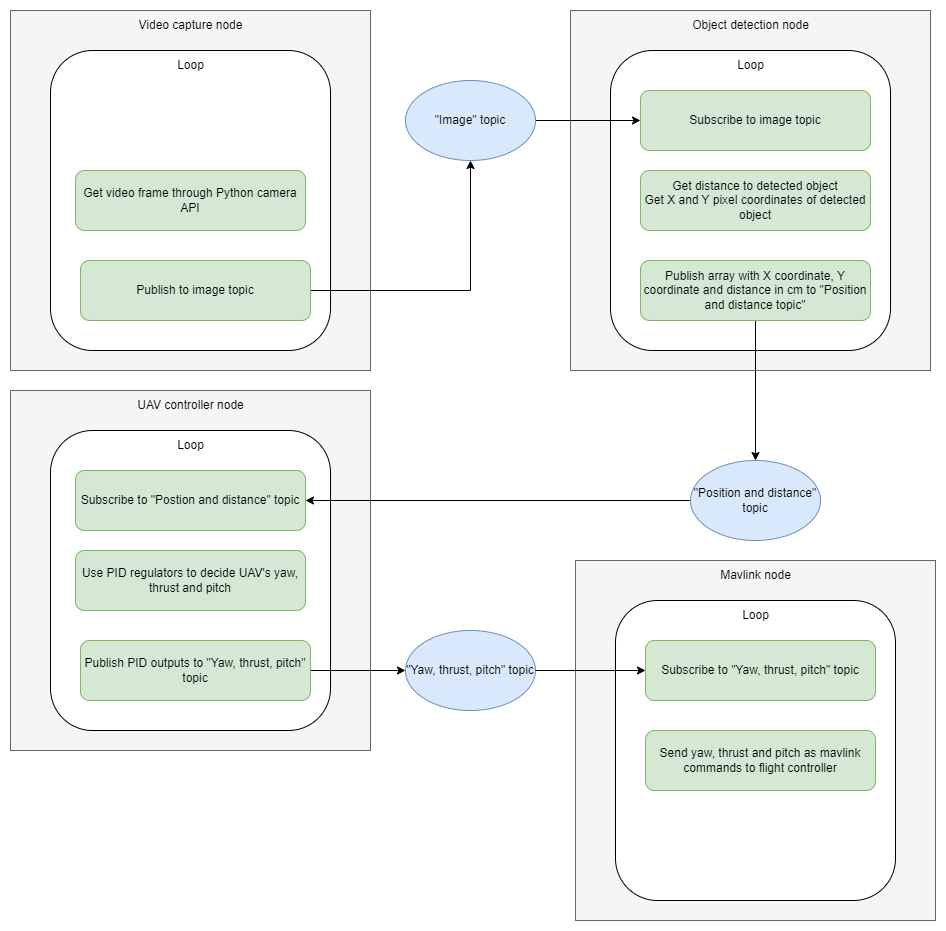
\includegraphics[width=\textwidth]{a_martinbilder/nodes.drawio.png}
    \caption{ROS2 node description}
    \label{fig:node_description}
\end{figure}

\subsection{UAV side project}

Throughout this study we have had ambition to fly a UAV with the ability to follow an object, as mentioned briefly in \ref{sub:accepted_architectures}. The “UAV controller node” and “Mavlink node” in figure \ref{fig:node_description} were made to achieve this goal. Results from real world testing on a UAV would be valuable when comparing the performance of our configurations. Unfortunately, we didn’t reach the point where we could launch a drone with the object following capability. We elaborate on this side project in appendix \ref{drone_impl}




\section{Drone architecture}

\begin{figure}[h]
    \centering
    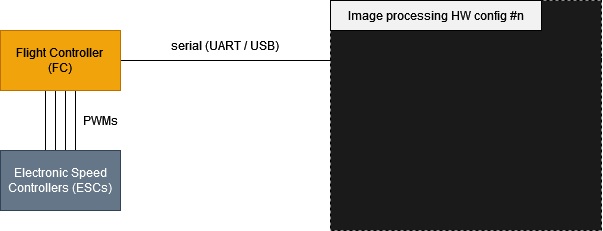
\includegraphics[width=\textwidth]{fig/arch_fc.png}
    \caption{Hardware architecture including the flight controller and ESCs}
    \label{fig:hw_fc}
\end{figure}

The configuration consists of a flight controller flashed with a firmware featuring the ability to receive relatively high-level commands from any image processing-stack and turn it into real, physical movement of a drone.\\
The firmware chosen for this Bachelor's thesis is the "ArduCopter"-firmware from the well-known ArduPilot\cite{documentation-ArduPilot} project, widely regarded as the best open-source flight controller firmware for UAV projects.\cite{firmware-FC} The high-level commands in question being sent is from the widely used MAVLink\cite{documentation-MAVLink} messaging protocol which can be received and transmitted through serial communications (UART / USB).

\subsection{Flight controller firmware setup}
The drone's flight controller has to be flashed with a version of ArduCopter and all necessary calibrations, ESC/motor-setup and tuning can be done through ArduPilot's official Mission Planner-application\cite{documentation-ArduPilot} installed on a desktop computer running Windows or Linux operating system.\\
The flight controller has to also be configured to accept the MAVLink messaging protocol on one of its serial Rx/Tx-ports, which also can be configured through Mission Planner.

\newpage

\subsection{Communication software setup}
The single-board computer in the image processing config-stack needs a way to transmit and recieve MAVLink messages to and from the flight controller. There exists readily available software solutions which can encode MAVLink messages and transmit them over a serial communications interface such as UART or USB.\\\\
Two software solutions were assessed during this Bachelor's thesis:\\
The "Pymavlink" Python-libraries\cite{github-Pymavlink} and the "MAVROS" ROS-package\cite{wiki-MAVROS}.\\\\
While both these solutions were assessed, only "Pymavlink" was actually implemented in a working configuration. This is due to the "MAVROS" ROS-package for the supported ROS 2 distributions (Foxy and Humble) still being in an alpha state\cite{github-MAVROS} as of the time of writing this report, and was therefore omitted.\\
More in-depth information and examples on MAVLink and "Pymavlink" can be found in \ref{MAVLink}.


\newpage

%\subsection{Test bench for distributed architectures}

%This section will cover the commonalities between the distributed architectures. \\

%Figure \ref{fig:dataflow} describes the test setup with internal interfaces. This setup contains all the components needed for a drone with autonomous capabilities, apart from the chassis and actuators which are not needed to measure data processing performance.
%As described in figure \ref{fig:dataflow} all four image processing configurations have the same output format. They publish distance and position data to ROS2 topics which the decision making module subscribes to. This common interface enables testing of the different image processing configurations without making any changes to the remaining modules that make up the drone.




\section{Exploring Use cases}

In this section of the research report, we delve into one of the primary motivations for this project, which is the potential applications of edge computing. Of particular interest is the use case involving drones, which encapsulates the entire spectrum of our work, ranging from the simulation of a drone via the Qualisys motion capture system to the actual construction and piloting of one.

In the following subsections, we will discuss the various tests conducted in our research, along with a detailed analysis of their respective outcomes.

\subsection{Qualisys and drone tracking}
The Qualisys motion capture system is a powerful tool that we use to pinpoint the exact location of the drone. It gives us real-time data on the drone's position in 3D space, with six degrees of freedom (6DOF). This means it can track the drone's movements forward and backward, up and down, left and right, as well as its rotations around three perpendicular axes. With this system, we can monitor and evaluate the drone's position in any environment, including a room. \cite{Qualisys}

\subsubsection{Drone tracking with Qualisys}
Qualisys is exceptionally efficient in tracking drones. It goes beyond merely determining the drone's location; Qualisys supplies accurate tracking data that captures the drone's nuanced movements in real-time. Specifically, we are focused on the yaw, x and y coordinates.
The yaw value helps us understand the drone's rotation around the vertical axis, while the x and y coordinates pinpoint the drone's position in three-dimensional space. By comparing this data with our drone location algorithm's output, we can assess the algorithm's accuracy and reliability. If there are discrepancies, we can refine our algorithm using this high-quality data, ensuring the drone's precise positioning and control.

\subsubsection{Drone position}
In order to calculate the drone position we need to get the distance data (denoted as $d$) from our image processing configurations, and we need to get the yaw (denoted as $\theta$) from the qualisys.
We use the yaw data to simulate magnetometer data we would get from the flightcontroller.
This testing have been done with a dummy drone with qualisys markers on the floor, so that we don't factor in the z axis.

We're essentially using a polar coordinate system with the object at the origin. In this system, a point is described by its distance from the origin, and its angle measured counterclockwise from a reference direction. For our specific problem, this angle is the drone's yaw.

Given this setup, the drone's x ($x_{\text{drone}}$) and y ($y_{\text{drone}}$) positions can be calculated by using trigonometric functions with the distance to the object and the drone's yaw. This calculation assumes that the object is at a location relative to origio, and the drone's yaw is defined as 0 when the drone is north of the object with the camera pointing south, increasing counterclockwise, and decreasing clockwise.

The equations to calculate the drone's position are as follows:

\begin{equation}
x_{\text{drone}} = x_{\text{object}} - d \cdot \sin(\theta)
\end{equation}

\begin{equation}
y_{\text{drone}} = y_{\text{object}} + d \cdot \cos(\theta)
\end{equation}

These equations account for the drone's distance from the object and its orientation. The trigonometric functions sin and cos help to decompose the total distance $d$ into x and y components, providing an estimate for the drone's position. After the estimation, we compare the calculated position with the true position. This allows us to gauge the accuracy of our algorithm. In addition, we plot these positions over time to visually assess the performance of our drone location algorithm.

\subsubsection{Test Results}

With the use of ROS2s get\_logger().info() and the plots generated, we were able to reliably read the test data from our calculations:

\begin{table}[h]
\centering
\resizebox{\textwidth}{!}{%
\begin{tabular}{|c|c|c|c|c|}
\hline
\textbf{Yaw (rad)} & \textbf{Distance to Object (cm)} & \textbf{Estimated Position(x,y)} & \textbf{True Position(x,y)} & \textbf{Difference (\%)}\\ \hline
-0.045 & 92 & (0.0395, 0.919) & (-0.086, 0.941) & 2.65 \\ \hline
1.524 & 88 & (-0.878, 0.0498) & (-0.984, -0.004) & 10.6 \\ \hline
3.015 & 80 & (-0.100, -0.793) & (-0.051, -0.810) & 1.43 \\ \hline
-1.581 & 86 & (0.859, -0.005) & (0.773, -0.017) & 11.1 \\ \hline
\end{tabular}%
}
\caption{Drone Position Testing Data}
\label{tab:qssTest}
\end{table}


The numbers we're discussing are average measurements taken from each yaw, using a still camera. These measurements consider all areas of the coordinate system that our Qualisys tracking system is adjusted to match. We compare our test data with the real coordinates from the Qualisys Tracking Manager (QTM). By finding the distance between each point, we can estimate the difference between them. This test was conducted with the object at the origin point (0,0).

\begin{figure}[!h]
    \centering
    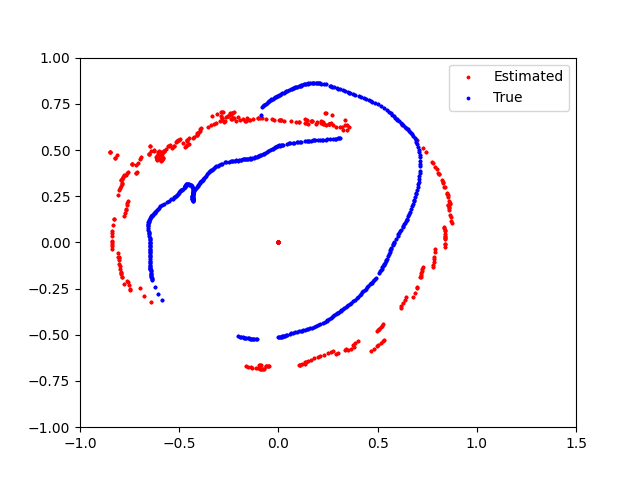
\includegraphics[scale=0.5]{sindrebilder/plotDronefinal.png}
    \caption{Estimated drone position vs Qualisys tracking data}
    \label{fig:qssPlot}
\end{figure}

Data from a moving camera, as shown in \ref{fig:qssPlot}, is not as accurate as the data from a still camera. This might be because the camera was placed half a meter above the ground, something we didn't account for in our tests. Even so, the results indicate that our function is working correctly, which is our main goal.

The testing was done with image processing configuration 4. And since the contours in the frames fluctuate a little from each time, this also factors in on the estimated values. 
\newpage

\subsubsection{ROS1 to ROS2}

The previous project by Local Hawk had utilized Qualisys for drone tracking, and we opted to use their existing codebase. However, this code was designed for ROS1, which required us to convert it to the newer ROS2 standard.

Initially, we contemplated using a bridge between ROS1 and ROS2. However, given that this bridge is still in the alpha phase and only supports standard ROS messages, it was not suited for our application as we were dealing with custom message types developed by Local Hawk. Hence, we decided to translate the ROS-related code from ROS1 to ROS2. We did not make any big changes to the calculations, other than setting some initial values, due to errors parsing the data into the calculation function.

A significant portion of the changes we made were the underlying architecture and methodology of ROS2, which diverges significantly from its predecessor.

The API client library has been changed, and they changed the architecture to be more object-oriented in ROS2. So everything from simple syntax to architecture have been changed. But most of the time was understanding how the ROS1 script worked.

One main challenge arose due to the Qualisys Tracking Manager (QTM) library's dependency on "Asyncio". Both Asyncio and ROS utilize event loops, which manage and distribute the execution of different tasks in an asynchronous programming environment.

This meant we needed to learn how the Asyncio event loop worked to understand what changes had been made. Essentially, these event loops allow multiple tasks to be executed concurrently, without the need for multi-threading or multi-processing. They achieve this by running one task until it needs to wait for an external event (like an I/O operation), then pausing that task and running another. This allows the program to utilize CPU time efficiently, as it can continue processing other tasks while waiting for the external event, instead of just sitting idle.\cite{loopRTS} \newpage

Instead of using the ROS2 spin function, we put the node into the Asyncio event loop. The Local Hawk team started this, but we had to change some parts of the code. You can see these changes in our code breakdown \hyperref[ch:ros1toros2]{here}.
